% Options for packages loaded elsewhere
% Options for packages loaded elsewhere
\PassOptionsToPackage{unicode}{hyperref}
\PassOptionsToPackage{hyphens}{url}
\PassOptionsToPackage{dvipsnames,svgnames,x11names}{xcolor}
%
\documentclass[
  spanish,
  a4paper,
  oneside]{scrbook}
\usepackage{xcolor}
\usepackage[top=25mm,bottom=25mm,left=30mm,right=20mm]{geometry}
\usepackage{amsmath,amssymb}
\setcounter{secnumdepth}{5}
\usepackage{iftex}
\ifPDFTeX
  \usepackage[T1]{fontenc}
  \usepackage[utf8]{inputenc}
  \usepackage{textcomp} % provide euro and other symbols
\else % if luatex or xetex
  \usepackage{unicode-math} % this also loads fontspec
  \defaultfontfeatures{Scale=MatchLowercase}
  \defaultfontfeatures[\rmfamily]{Ligatures=TeX,Scale=1}
\fi
\usepackage{lmodern}
\ifPDFTeX\else
  % xetex/luatex font selection
  \setmainfont[]{Times New Roman}
\fi
% Use upquote if available, for straight quotes in verbatim environments
\IfFileExists{upquote.sty}{\usepackage{upquote}}{}
\IfFileExists{microtype.sty}{% use microtype if available
  \usepackage[]{microtype}
  \UseMicrotypeSet[protrusion]{basicmath} % disable protrusion for tt fonts
}{}
\makeatletter
\@ifundefined{KOMAClassName}{% if non-KOMA class
  \IfFileExists{parskip.sty}{%
    \usepackage{parskip}
  }{% else
    \setlength{\parindent}{0pt}
    \setlength{\parskip}{6pt plus 2pt minus 1pt}}
}{% if KOMA class
  \KOMAoptions{parskip=half}}
\makeatother
% Make \paragraph and \subparagraph free-standing
\makeatletter
\ifx\paragraph\undefined\else
  \let\oldparagraph\paragraph
  \renewcommand{\paragraph}{
    \@ifstar
      \xxxParagraphStar
      \xxxParagraphNoStar
  }
  \newcommand{\xxxParagraphStar}[1]{\oldparagraph*{#1}\mbox{}}
  \newcommand{\xxxParagraphNoStar}[1]{\oldparagraph{#1}\mbox{}}
\fi
\ifx\subparagraph\undefined\else
  \let\oldsubparagraph\subparagraph
  \renewcommand{\subparagraph}{
    \@ifstar
      \xxxSubParagraphStar
      \xxxSubParagraphNoStar
  }
  \newcommand{\xxxSubParagraphStar}[1]{\oldsubparagraph*{#1}\mbox{}}
  \newcommand{\xxxSubParagraphNoStar}[1]{\oldsubparagraph{#1}\mbox{}}
\fi
\makeatother


\usepackage{longtable,booktabs,array}
\usepackage{calc} % for calculating minipage widths
% Correct order of tables after \paragraph or \subparagraph
\usepackage{etoolbox}
\makeatletter
\patchcmd\longtable{\par}{\if@noskipsec\mbox{}\fi\par}{}{}
\makeatother
% Allow footnotes in longtable head/foot
\IfFileExists{footnotehyper.sty}{\usepackage{footnotehyper}}{\usepackage{footnote}}
\makesavenoteenv{longtable}
\usepackage{graphicx}
\makeatletter
\newsavebox\pandoc@box
\newcommand*\pandocbounded[1]{% scales image to fit in text height/width
  \sbox\pandoc@box{#1}%
  \Gscale@div\@tempa{\textheight}{\dimexpr\ht\pandoc@box+\dp\pandoc@box\relax}%
  \Gscale@div\@tempb{\linewidth}{\wd\pandoc@box}%
  \ifdim\@tempb\p@<\@tempa\p@\let\@tempa\@tempb\fi% select the smaller of both
  \ifdim\@tempa\p@<\p@\scalebox{\@tempa}{\usebox\pandoc@box}%
  \else\usebox{\pandoc@box}%
  \fi%
}
% Set default figure placement to htbp
\def\fps@figure{htbp}
\makeatother


% definitions for citeproc citations
\NewDocumentCommand\citeproctext{}{}
\NewDocumentCommand\citeproc{mm}{%
  \begingroup\def\citeproctext{#2}\cite{#1}\endgroup}
\makeatletter
 % allow citations to break across lines
 \let\@cite@ofmt\@firstofone
 % avoid brackets around text for \cite:
 \def\@biblabel#1{}
 \def\@cite#1#2{{#1\if@tempswa , #2\fi}}
\makeatother
\newlength{\cslhangindent}
\setlength{\cslhangindent}{1.5em}
\newlength{\csllabelwidth}
\setlength{\csllabelwidth}{3em}
\newenvironment{CSLReferences}[2] % #1 hanging-indent, #2 entry-spacing
 {\begin{list}{}{%
  \setlength{\itemindent}{0pt}
  \setlength{\leftmargin}{0pt}
  \setlength{\parsep}{0pt}
  % turn on hanging indent if param 1 is 1
  \ifodd #1
   \setlength{\leftmargin}{\cslhangindent}
   \setlength{\itemindent}{-1\cslhangindent}
  \fi
  % set entry spacing
  \setlength{\itemsep}{#2\baselineskip}}}
 {\end{list}}
\usepackage{calc}
\newcommand{\CSLBlock}[1]{\hfill\break\parbox[t]{\linewidth}{\strut\ignorespaces#1\strut}}
\newcommand{\CSLLeftMargin}[1]{\parbox[t]{\csllabelwidth}{\strut#1\strut}}
\newcommand{\CSLRightInline}[1]{\parbox[t]{\linewidth - \csllabelwidth}{\strut#1\strut}}
\newcommand{\CSLIndent}[1]{\hspace{\cslhangindent}#1}

\ifLuaTeX
\usepackage[bidi=basic]{babel}
\else
\usepackage[bidi=default]{babel}
\fi
\ifPDFTeX
\else
\babelfont{rm}[]{Times New Roman}
\fi
% get rid of language-specific shorthands (see #6817):
\let\LanguageShortHands\languageshorthands
\def\languageshorthands#1{}


\setlength{\emergencystretch}{3em} % prevent overfull lines

\providecommand{\tightlist}{%
  \setlength{\itemsep}{0pt}\setlength{\parskip}{0pt}}



 


% ---------- Paquetes tipograficos y microajustes ----------
\usepackage{microtype}        % mejor interletrado y justificado
\usepackage{csquotes}         % comillas tipograficas
\usepackage{iftex}
\ifPDFTeX\else
  % Seleccion de fuentes solo cuando XeTeX/LuaTeX esta disponible.
  \IfFontExistsTF{Times New Roman}{
    \setmainfont{Times New Roman}
  }{
    \IfFontExistsTF{TeX Gyre Termes}{
      \setmainfont{TeX Gyre Termes}
    }{
      \IfFontExistsTF{Latin Modern Roman}{\setmainfont{Latin Modern Roman}}{}
    }
  }
  \IfFontExistsTF{Times New Roman}{
    \setsansfont{Times New Roman}
  }{
    \IfFontExistsTF{TeX Gyre Heros}{
      \setsansfont{TeX Gyre Heros}
    }{
      \IfFontExistsTF{Latin Modern Sans}{\setsansfont{Latin Modern Sans}}{}
    }
  }
  \IfFontExistsTF{Times New Roman}{
    \setmonofont{Times New Roman}
  }{
    \IfFontExistsTF{TeX Gyre Cursor}{
      \setmonofont{TeX Gyre Cursor}
    }{
      \IfFontExistsTF{Latin Modern Mono}{\setmonofont{Latin Modern Mono}}{}
    }
  }
\fi
\usepackage{enumitem}         % listas compactas
\setlist{itemsep=.2em, topsep=.2em}

% ---------- KOMA-Script: estilo de titulos y espaciado ----------
\KOMAoptions{
  headings=big,
  parskip=half,
  fontsize=12pt,
  appendixprefix=true
}
\setlength{\parindent}{1.5em}
\setlength{\parskip}{0.6em}
\usepackage{indentfirst}
\usepackage{setspace}
\setstretch{1.5}


% ---------- Encabezados y pies (scrlayer-scrpage) ----------
\usepackage[automark,headsepline]{scrlayer-scrpage}
\clearpairofpagestyles
\automark[chapter]{chapter}
\ihead{\pagemark}
\ohead{\itshape\headmark}
\setheadsepline{0.4pt}
\renewcommand*{\chaptermarkformat}{}
\renewcommand*{\chapterpagestyle}{scrheadings}
\pagestyle{scrheadings}
\makeatletter
\let\ps@plain\ps@scrheadings
\makeatother
\cfoot{}

% ---------- Hipervinculos mas sobrios ----------
\usepackage{hyperref}
\hypersetup{
  colorlinks=true,
  linkcolor=blue,
  citecolor=blue,
  urlcolor=blue,
  pdfauthor={\@author},
  pdftitle={\@title}
}

% ---------- Leyendas de figuras/tablas ----------
\usepackage[labelfont=bf,textfont=it]{caption}
\captionsetup{
  skip=8pt
}

% ---------- Tabla de contenidos ----------
\KOMAoptions{toc=graduated}
\RedeclareSectionCommand[tocnumwidth=3em]{chapter}
\RedeclareSectionCommand[tocindent=3.25em,tocnumwidth=2.8em]{section}
\RedeclareSectionCommand[tocindent=6.5em,tocnumwidth=2.5em]{subsection}
\makeatletter
\newcommand*{\tocdotfill}{\leavevmode\leaders\hbox to .6em{\hss.\hss}\hfill}
\makeatother
\RedeclareSectionCommand[toclinefill=\tocdotfill]{chapter}
\RedeclareSectionCommand[toclinefill=\tocdotfill]{section}
\RedeclareSectionCommand[toclinefill=\tocdotfill]{subsection}
\renewcommand*{\contentsname}{Tabla de contenido}
\setkomafont{chapterentry}{\normalfont}
\setkomafont{chapterentrypagenumber}{\normalfont}

% ---------- Viudas/Huerfanas y cortes de pagina ----------
\clubpenalty=10000
\widowpenalty=10000
\displaywidowpenalty=10000

% ---------- Entorno abstract para scrbook ----------
\providecommand{\abstractname}{Resumen}
\makeatletter
\@ifundefined{abstract}{
  \newenvironment{abstract}{
    \cleardoublepage
    \thispagestyle{plain}
    \null\vfill
    \begin{center}
      {\bfseries\Large \abstractname\par}
    \end{center}\vspace{1em}
    \begingroup
  }{
    \par\endgroup
    \vfill\null
    \cleardoublepage
  }
}{}
\makeatother

% ---------- Soporte de subtitulo desde YAML ----------
\makeatletter
\providecommand{\subtitle}[1]{\gdef\@subtitle{#1}}
\providecommand{\@subtitle}{}
\makeatother

% --- Desactivar portada y abstract automaticos de Pandoc (PDF) ---
\AtBeginDocument{\let\maketitle\relax}
\renewenvironment{abstract}{}{}
\providecommand{\appendixname}{}
\providecommand{\appendixtocname}{}
\providecommand{\appendixpagename}{}
\renewcommand*{\appendixname}{Anexo}
\renewcommand*{\appendixtocname}{Anexos}
\renewcommand*{\appendixpagename}{Anexos}


% ---------- Indicadores para LOF/LOT condicionales ----------
\newif\iffacsofigexists
\newif\iffacsotableexists
\InputIfFileExists{\jobname.facsoflags}{}{}
\newwrite\FacsoFlagStream
\AtEndDocument{%
  \immediate\openout\FacsoFlagStream=\jobname.facsoflags
  \ifnum\value{figure}>0
    \immediate\write\FacsoFlagStream{\string\facsofigexiststrue}
  \else
    \immediate\write\FacsoFlagStream{\string\facsofigexistsfalse}
  \fi
  \ifnum\value{table}>0
    \immediate\write\FacsoFlagStream{\string\facsotableexiststrue}
  \else
    \immediate\write\FacsoFlagStream{\string\facsotableexistsfalse}
  \fi
  \immediate\closeout\FacsoFlagStream
}
\hypersetup{
  colorlinks=true,
  linkcolor=blue,
  urlcolor=blue,
  citecolor=blue
}
\makeatletter
\@ifpackageloaded{bookmark}{}{\usepackage{bookmark}}
\makeatother
\makeatletter
\@ifpackageloaded{caption}{}{\usepackage{caption}}
\AtBeginDocument{%
\ifdefined\contentsname
  \renewcommand*\contentsname{Tabla de contenidos}
\else
  \newcommand\contentsname{Tabla de contenidos}
\fi
\ifdefined\listfigurename
  \renewcommand*\listfigurename{Listado de Figuras}
\else
  \newcommand\listfigurename{Listado de Figuras}
\fi
\ifdefined\listtablename
  \renewcommand*\listtablename{Listado de Tablas}
\else
  \newcommand\listtablename{Listado de Tablas}
\fi
\ifdefined\figurename
  \renewcommand*\figurename{Lista de figuras}
\else
  \newcommand\figurename{Lista de figuras}
\fi
\ifdefined\tablename
  \renewcommand*\tablename{Lista de tablas}
\else
  \newcommand\tablename{Lista de tablas}
\fi
}
\@ifpackageloaded{float}{}{\usepackage{float}}
\floatstyle{ruled}
\@ifundefined{c@chapter}{\newfloat{codelisting}{h}{lop}}{\newfloat{codelisting}{h}{lop}[chapter]}
\floatname{codelisting}{Listado}
\newcommand*\listoflistings{\listof{codelisting}{Listado de Listados}}
\makeatother
\makeatletter
\makeatother
\makeatletter
\@ifpackageloaded{caption}{}{\usepackage{caption}}
\@ifpackageloaded{subcaption}{}{\usepackage{subcaption}}
\makeatother
\usepackage{bookmark}
\IfFileExists{xurl.sty}{\usepackage{xurl}}{} % add URL line breaks if available
\urlstyle{same}
\hypersetup{
  pdftitle={Ansiedad matemática y rendimiento en estudiantes chilenos},
  pdfauthor={Katherine Aravena Herrera},
  pdflang={es},
  colorlinks=true,
  linkcolor={black},
  filecolor={Maroon},
  citecolor={blue},
  urlcolor={blue},
  pdfcreator={LaTeX via pandoc}}


\title{Ansiedad matemática y rendimiento en estudiantes chilenos}
\usepackage{etoolbox}
\makeatletter
\providecommand{\subtitle}[1]{% add subtitle to \maketitle
  \apptocmd{\@title}{\par {\large #1 \par}}{}{}
}
\makeatother
\subtitle{Diferencias socioeconómicas en un sistema escolar altamente
estratificado}
\author{Katherine Aravena Herrera}
\date{1 de diciembre de 2025}
\begin{document}
\frontmatter
\maketitle

% --- title-pdf.tex personalizado para portada formal ---
\newcommand{\CoverFont}{
  \ifdefined\fontspec
    \fontspec{Times New Roman}
  \else
    \fontfamily{ptm}\selectfont
  \fi
}
\makeatletter
\providecommand{\subtitle}[1]{\gdef\@subtitle{#1}}
\providecommand{\@subtitle}{}
\providecommand{\frontmattercontext}{}
\providecommand{\advisorname}{}
\providecommand{\advisorlabel}{Profesor guia:}
\providecommand{\frontmatterlocation}{}
\InputIfFileExists{includes/cover-config.tex}{}{}

\newcommand{\PrintTitle}{%
  {\CoverFont\fontsize{24pt}{28pt}\selectfont \@title\par}%
}
\newcommand{\PrintSubtitle}{%
  \begingroup
  \edef\temp{\detokenize{\@subtitle}}%
  \ifx\temp\empty\relax
    % sin subtitulo
  \else
    {\CoverFont\large \@subtitle\par}%
  \fi
  \endgroup
}
\newcommand{\PrintAuthor}{%
  {\CoverFont\Large\bfseries \@author\par}%
}
\newcommand{\PrintDate}{%
  {\CoverFont\small \@date\par}%
}
\makeatother

\begin{titlepage}
\thispagestyle{empty}
\begin{center}
\CoverFont
\vspace*{10mm}

% Logo o imagen institucional

\includegraphics[width=0.35\textwidth]{assets/cover.png}\par
\vspace{12mm}

% Titulo y subtitulo
\PrintTitle
\vspace{6mm}
\PrintSubtitle

\vspace{22mm}
\begingroup
\edef\temp{\detokenize{\frontmattercontext}}%
\ifx\temp\empty\relax
  % sin contexto adicional
\else
  {\normalsize \CoverFont \frontmattercontext\par}%
\fi
\endgroup

\vspace{18mm}
\PrintAuthor

\vspace{16mm}
\begingroup
\edef\temp{\detokenize{\advisorname}}%
\ifx\temp\empty\relax
  % sin tutor
\else
  \rule{0.45\textwidth}{0.4pt}\par
  {\small \CoverFont \advisorlabel\ \advisorname\par}%
\fi
\endgroup

\vfill
\begingroup
\edef\temp{\detokenize{\frontmatterlocation}}%
\ifx\temp\empty\relax
  % sin ubicacion
\else
  {\small \CoverFont \frontmatterlocation\par}%
\fi
\endgroup
\PrintDate

\end{center}
\end{titlepage}

% Preliminares (numeros romanos) y estilo simple
\frontmatter
\pagestyle{scrheadings}

\setcounter{tocdepth}{2} % (o 1/3 segun prefieras)
\tableofcontents
\iffacsofigexists
  \cleardoublepage
  \listoffigures
\fi
\cleardoublepage


\mainmatter
\bookmarksetup{startatroot}

\chapter*{Presentación}\label{presentaciuxf3n}
\addcontentsline{toc}{chapter}{Presentación}

\markboth{Presentación}{Presentación}

\small\textbf{Palabras clave: } Ansiedad matemática; Rendimiento en
Matemática; Nivel socioeconómico; Desigualdad educativa; Modelos
multinivel. \normalsize

La presente investigación se enmarca en mí seminario para optar al grado
de Licenciatura en Sociología de la Universidad de Chile. El trabajo fue
desarrollado en el Departamento de Sociología y cuenta con la
supervisión del profesor guía, Dr.~Juan Carlos Castillo Valenzuela.

\bookmarksetup{startatroot}

\chapter{Introducción}\label{introducciuxf3n}

En el sistema educativo chileno persiste una brecha por nivel
socioeconómico en los aprendizajes de Matemática: a mayor nivel
socioeconómico de las y los estudiantes, mayor tiende a ser su
rendimiento en pruebas estandarizadas
(\citeproc{ref-mineduc2023pisa}{Ministerio de Educación de Chile \&
Unidad de Currículum y Evaluación, 2023};
\citeproc{ref-mizala2012chile}{Mizala \& Torche, 2012};
\citeproc{ref-oecd2023pisa}{OECD, 2023b},
\citeproc{ref-oecd2023chile}{2023a}). Este patrón se inscribe en una
estructura escolar chilena históricamente segregada por origen social y
recursos, en el que la composición socioeconómica de los
establecimientos condiciona oportunidades, expectativas y el clima de
aprendizaje (\citeproc{ref-agencia2023resultados}{Agencia de Calidad de
la Educación, 2023c}; \citeproc{ref-mizala2012chile}{Mizala \& Torche,
2012}). La literatura, tanto nacional como internacional, ha documentado
de manera consistente estos efectos de contexto escolar, mostrando que
las características individuales de los estudiantes no son el único
factor relevante, sino que también la concentración de recursos, que se
traduce en ventajas y desventajas de cada establecimiento escolar
(\citeproc{ref-mizala2012chile}{Mizala \& Torche, 2012};
\citeproc{ref-oecd2023pisa}{OECD, 2023b},
\citeproc{ref-oecd2023chile}{2023a}). En este sentido, se ha investigado
ampliamente sobre cuán grandes son las diferencias de aprendizaje según
el origen social, pero mucho menos sobre qué mecanismos emocionales y
cognitivos, dentro de las clases de Matemática, explican y conectan ese
origen social con los resultados de rendimiento
(\citeproc{ref-ashcraft2002}{Ashcraft, 2002};
\citeproc{ref-ashcraft2009}{Ashcraft \& Moore, 2009};
\citeproc{ref-Pekrun2006}{Pekrun, 2006a}).

En este marco, la ansiedad hacia las Matemáticas aparece como un factor
psicológico clave para comprender cómo los estudiantes se han
relacionado con esta asignatura. De manera general, se entiende como un
conjunto de emociones negativas, como tensión, preocupación, incomodidad
o temor, que las personas experimentan al anticipar o enfrentar tareas
que involucran Matemática en contextos de clase, estudio o evaluación
(\citeproc{ref-szucs2020}{Szűcs \& Mammarella, 2020}). La evidencia
disponible muestra que esta experiencia emocional se asocia
sistemáticamente con resultados académicos desfavorables, como una menor
satisfacción con la asignatura, menor intención de continuar y
profundizar en el estudio de las Matemáticas, niveles más bajos de
autoeficacia y un rendimiento académico inferior a lo largo de la
trayectoria escolar (\citeproc{ref-ashcraft2002}{Ashcraft, 2002};
\citeproc{ref-ashcraft2009}{Ashcraft \& Moore, 2009};
\citeproc{ref-hembree1990}{Hembree, 1990a}). Desde esta perspectiva, la
ansiedad no solo acompaña el bajo rendimiento, sino que puede
convertirse en un mecanismo que lo reproduce y profundiza en el tiempo
(\citeproc{ref-ashcraft2002}{Ashcraft, 2002};
\citeproc{ref-Carey2019}{Carey et~al., 2019};
\citeproc{ref-hembree1990}{Hembree, 1990a}). Esto sitúa a la ansiedad
matemática en un lugar estratégico para entender cómo las estructuras de
desigualdad se reproduce en experiencias subjetivas de aprendizaje, dado
que el problema no se reduce a saber o no saber Matemática, sino que
también incluye la forma en que el estudiantado se siente al enfrentarse
esta disciplina (\citeproc{ref-ashcraft2002}{Ashcraft, 2002};
\citeproc{ref-pekrun2006}{Pekrun, 2006b}). Se trata de un punto de
intersección entre cognición y afecto, que involucra creencias sobre la
propia capacidad, sentimientos de amenaza o inseguridad frente al
fracaso y procesos cognitivos que se ven interferidos cuando la persona
se siente observada o evaluada, como la memoria de trabajo y la atención
sostenida (\citeproc{ref-Young2012}{Young et~al., 2012a}).

Junto a lo anterior, también que la ansiedad matemática no se distribuye
de manera homogénea entre grupos sociales, documentado de manera
consistente que niñas y mujeres tienden a reportar niveles más altos de
ansiedad matemática que niños y hombres (\citeproc{ref-bieg2015}{Bieg
et~al., 2015}; \citeproc{ref-devine2012}{Devine et~al., 2012};
\citeproc{ref-goetz2013}{Goetz et~al., 2013};
\citeproc{ref-hembree1990}{Hembree, 1990a}; \citeproc{ref-hyde1990}{Hyde
et~al., 1990}; \citeproc{ref-richardson1972}{Richardson \& Suinn,
1972}). Estas diferencias se han vinculado con estereotipos de género
sobre quién es considerado como naturalmente bueno para las matemáticas
y con prácticas escolares y familiares que refuerzan expectativas
diferenciadas respecto del desempeño y la elección de trayectorias
formativas (\citeproc{ref-bieg2015}{Bieg et~al., 2015};
\citeproc{ref-goetz2013}{Goetz et~al., 2013}). Aunque el foco de la
presente investigación no está en las brechas de género, este
antecedente refuerza la idea de que la ansiedad matemática no es una
característica puramente individual, sino que se estructura en torno a
posiciones sociales como género u origen socioeconómico y se alimenta de
las interacciones y climas que se construyen en las aulas
(\citeproc{ref-devine2012}{Devine et~al., 2012};
\citeproc{ref-goetz2013}{Goetz et~al., 2013}). En un sistema escolar tan
estratificado como el chileno, se espera que la ansiedad matemática
también se distribuya de forma desigual según el nivel socioeconómico y
se exprese con distinta intensidad en distintos tipos de
establecimientos (\citeproc{ref-agencia2023resultados}{Agencia de
Calidad de la Educación, 2023c}; \citeproc{ref-mizala2012chile}{Mizala
\& Torche, 2012}).

En Chile, la política educativa reciente ha impulsando el bienestar y la
socioemocionalidad como dimensiones prioritarias de la agenda escolar en
el marco de la reactivación educativa tras la pandemia, a través de
iniciativas que combinan apoyo académico y socioemocional
(\citeproc{ref-oecd2023chile}{OECD, 2023a}). Al mismo tiempo, la
evidencia disponible indica que los choques asociados al COVID-19 han
intensificado las desigualdades de logro, con pérdidas mayores en
Matemática y efectos particularmente marcados en estudiantes de menor
nivel socioeconómico (\citeproc{ref-Jakubowski2025-qv}{Jakubowski
et~al., 2025};
\citeproc{ref-MenesesOrtegaKuzmanicValenzuela2025}{Meneses et~al.,
2025}). PISA 2022 confirma que el gradiente socioeconómico en Matemática
no solo persiste, sino que se mantiene entre los más altos de la OCDE
(\citeproc{ref-oecd2023pisa}{OECD, 2023b},
\citeproc{ref-oecd2023chile}{2023a}). En este escenario, identificar
mecanismos psicoeducativos que puedan ser objeto de intervención, como
la ansiedad hacia las Matemáticas, resulta especialmente relevante. A
diferencia del origen social o de la estructura del sistema, las
emociones y creencias que se construyen en el aula pueden ser trabajadas
mediante prácticas de enseñanza, evaluación y acompañamiento pedagógico
(\citeproc{ref-black1998assessment}{Black \& Wiliam, 1998};
\citeproc{ref-carey2016}{Carey et~al., 2016};
\citeproc{ref-pekrun2006}{Pekrun, 2006b}). Considerando lo anterior, la
pregunta que se abre no es solo si la ansiedad matemática se asocia al
rendimiento, sino cómo interactúa con la desigualdad socioeconómica y
con los contextos escolares en los que los estudiantes aprenden.

Hasta ahora, la linvestigación sobre ansiedad matemática ha estado
fuertemente anclada en la psicología educacional, con énfasis en
factores individuales como el autoconcepto, la autoeficacia o la
ansiedad frente a pruebas (\citeproc{ref-ashcraft2002}{Ashcraft, 2002};
\citeproc{ref-goetz2013}{Goetz et~al., 2013};
\citeproc{ref-young2012}{Young et~al., 2012b}), mientras que, en los
estudios sobre desigualdad educativa y segregación escolar, la
sociología y la economía de la educación se han centrado en
determinantes estructurales y de política educativa como la segregación,
la selección y el financiamiento
(\citeproc{ref-agencia2023resultados}{Agencia de Calidad de la
Educación, 2023c}; \citeproc{ref-mizala2012chile}{Mizala \& Torche,
2012}).Siguiendo esta línea, se ha explorado poco trabajos que combinen
ambas perspectivas, integrando la ansiedad matemática como mecanismo
explicativo dentro de modelos que consideren simultáneamente origen
social, contexto escolar y rendimiento (\citeproc{ref-carey2016}{Carey
et~al., 2016}). Esta separación entre el estudio de las desigualdades
estructurales y el de los mecanismos emocionales es precisamente el
vacío que este estudio busca abordar.

Como se menciono anteriomente, el presente estudio busca articular estos
campos y abordar la desigualdad en Matemática desde una perspectiva que
combine determinantes estructurales, contextuales y psicoeducativos. El
argumento central que guía la investigación es que la ansiedad hacia las
Matemáticas constituye un mecanismo clave en la relación entre el nivel
socioeconómico del estudiantado y su rendimiento, y que la magnitud y
forma de este efecto dependen del contexto escolar en el que se sitúa
cada estudiante. En particular, se plantea que la ansiedad matemática no
solo se distribuye de forma desigual según el nivel socioeconómico, sino
que su impacto sobre el desempeño puede verse amplificado en escuelas
con alta concentración de desventajas y climas emocionales más tensos, y
atenuado en establecimientos con mayores recursos y climas que promueven
el apoyo, la participación y la resignificación del error
(\citeproc{ref-fraser2012classroom}{Fraser, 2012};
\citeproc{ref-hattie2009visible}{Hattie, 2009a}). Así, la ansiedad
matemática puede operar como mediadora, al explicar parte de la
asociación entre nivel socioeconómico y resultados, y también como
moderadora, al condicionar la fuerza de dicha asociación según la
composición y el clima del establecimiento.

A partir de este marco, el estudio se apoya en la muestra chilena de
PISA 2022. Esta base de datos permite, por una parte, contar con una
medida estandarizada del rendimiento en Matemática y con un índice
socioeconómico cultural del hogar y, por otra, disponer de indicadores
de ansiedad matemática y de información suficiente para construir
medidas de composición socioeconómica y de clima de ansiedad a nivel de
establecimiento (\citeproc{ref-mineduc2023pisa}{Ministerio de Educación
de Chile \& Unidad de Currículum y Evaluación, 2023};
\citeproc{ref-oecd2023pisa}{OECD, 2023b}). El uso de modelos multinivel
resulta especialmente pertinente, en tanto reconoce la estructura
jerárquica de los datos, con estudiantes anidados en escuelas, y permite
estimar simultáneamente efectos individuales y contextuales, así como
interacciones entre ellos (\citeproc{ref-hox2017multilevel}{Hox et~al.,
2017a}). Desde un punto de vista metodológico, esta aproximación hace
posible examinar de manera más precisa en qué medida la ansiedad
matemática ayuda a explicar las brechas por nivel socioeconómico y cómo
se modifica su efecto según el tipo de escuela y el clima que se vive en
ella.

A partir del problema y argumento expuesto, la investigación se organiza
en torno a la siguientes preguntas y objetivo general y específicos:

\section{Preguntas de
investigación}\label{preguntas-de-investigaciuxf3n}

\begin{enumerate}
\def\labelenumi{\arabic{enumi}.}
\item
  ¿En qué medida la relación entre el nivel socioeconómico del
  estudiante y su rendimiento en Matemática se ve afectada por la
  ansiedad hacia las Matemáticas?
\item
  ¿Cómo varía este efecto según la composición socioeconómica y el clima
  de ansiedad matemática del establecimiento en estudiantes chilenos el
  año 2022?
\end{enumerate}

\section{Objetivo general}\label{objetivo-general}

Analizar en qué medida la relación entre el nivel socioeconómico del
estudiante y su rendimiento en Matemática se ve afectada por la ansiedad
ante la matemática a nivel individual, y cómo cambia según la
composición socioeconómica y el clima de ansiedad matemática del
establecimiento, en la muestra chilena de PISA 2022.

\section{Objetivos específicos}\label{objetivos-especuxedficos}

\begin{enumerate}
\def\labelenumi{\arabic{enumi}.}
\item
  Determinar la relación entre el nivel socioeconómico del estudiante y
  su rendimiento en Matemática.
\item
  Analizar la influencia de la ansiedad ante la matemática sobre el
  rendimiento en Matemática, incluyendo la evaluación de posibles
  comportamientos no lineales de la ansiedad.
\item
  Examinar en qué medida la composición socioeconómica del
  establecimiento y el clima de ansiedad matemática de la escuela
  modifican (atenúan o amplifican) el efecto de la ansiedad individual
  sobre el rendimiento y la relación entre el nivel socioeconómico del
  estudiante y su desempeño en Matemática.
\end{enumerate}

\bookmarksetup{startatroot}

\chapter{Antecedentes conceptuales y
empíricos}\label{antecedentes-conceptuales-y-empuxedricos}

\section{Desigualdades y brecha socioeconómica en el rendimiento en
Matemática}\label{desigualdades-y-brecha-socioeconuxf3mica-en-el-rendimiento-en-matemuxe1tica}

La literatura internacional y chilena ha avanzado significativamente en
identificar los mecanismos mediante los cuales el origen social se
traduce en diferencias de logro. En PISA 2022, Chile se ubica entre los
países con mayores brechas de desempeño en Matemática por nivel
socioeconómico, incluso controlando otras características individuales y
escolares
(\citeproc{ref-repec:eee:injoed:v:92:y:2022:i:c:s0738059322000785}{Ceron
et~al., 2022}). Este gradiente se observa de forma reiterada en diversas
rondas de evaluaciones, lo que sugiere la presencia de mecanismos
estructurales persistentes que vinculan el origen social con los logros
en Matemática
(\citeproc{ref-Global_Education_Monitoring_Report_Team2020-xq}{Global
Education Monitoring Report Team et~al., 2020};
\citeproc{ref-Neuman2022}{Neuman, 2022}).

En el caso chileno, evidencia reciente muestra la persistencia de
brechas de logro asociadas al origen social y la posición de clase
(\citeproc{ref-MenesesOrtegaKuzmanicValenzuela2025}{Meneses et~al.,
2025}). Estudiantes de menor nivel socioeconómico tienden a concentrarse
en establecimientos con peores resultados promedio y menor dotación de
recursos, mientras que aquellos de origen favorecido asisten a escuelas
que combinan mejores resultados académicos, mejor infraestructura y
docentes con mayor experiencia (\citeproc{ref-UNESCO2020}{UNESCO,
2020}). Informes de la Agencia de Calidad de la Educación
(\citeproc{ref-Agencia2023}{2023b}) confirman que estas brechas se
reproducen curso a curso, de modo que el sistema escolar opera más como
mecanismo de reproducción de la desigualdad que como instancia de
compensación. A nivel comparado, Chile se mantiene entre los países de
la OCDE con mayores niveles de desigualdad educativa, tanto en
resultados de aprendizaje como en acceso a trayectorias diferenciadas
(\citeproc{ref-CeronBolWerfhorst2022}{Cerón et~al., 2022}).

Desde la sociología de la educación, una parte central de la literatura
enfatiza mecanismos asociados al capital cultural y la reproducción
social. Bourdieu \& Passeron (\citeproc{ref-BourdieuPasseron1977}{1977})
sostienen que la escuela legitima como mérito las disposiciones
culturales propias de las clases medias y altas, naturalizando las
ventajas de quienes poseen habitus y capital cultural acordes a los
códigos escolares. El éxito escolar se presenta como producto del
esfuerzo individual, pero descansa en disposiciones adquiridas en el
hogar, por ejemplo, el manejo del lenguaje académico o la familiaridad
con las expectativas de los profesores
(\citeproc{ref-Bourdieu2000}{Bourdieu, 2000}). Siguiendo esta línea, la
brecha en Matemática refleja también la distancia entre los habitus de
las y los estudiantes y las formas de relación con el conocimiento que
la escuela privilegia (\citeproc{ref-Bourdieu1979}{Bourdieu, 1979},
\citeproc{ref-Bourdieu2000}{2000};
\citeproc{ref-BourdieuPasseron1977}{Bourdieu \& Passeron, 1977}).

Siguiendo esta línea, Lareau (\citeproc{ref-Lareau2003}{2003})
complementa este enfoque al mostrar cómo los estilos de crianza
diferenciados por clase, producen desigualdades en vocabulario, manejo
de normas institucionales y habilidades para desenvolverse en el sistema
educativo. En familias de clases medias y altas se fomenta la
participación en actividades extracurriculares y el razonamiento verbal,
enseñando a argumentar y pedir explicaciones, mientras que en contextos
de clase trabajadora la socialización cotidiana está menos orientada por
la lógica escolar (\citeproc{ref-Lareau2003}{Lareau, 2003}). En
Matemática, estas diferencias se traducen en la disponibilidad de apoyo
familiar, materiales didácticos y oportunidades para naturalizar el
razonamiento formal (\citeproc{ref-HascoetGiaconiJamain2021}{Hascoët
et~al., 2021}). En consecuencia, la brecha de rendimiento no se explica
sólo por carencias materiales, sino también por desigualdades en las
formas de relación con el conocimiento y las instituciones
(\citeproc{ref-Calarco2020}{Calarco, 2020}). Estudiantes de mayor nivel
socioeconómico acceden a escuelas más dotadas y llegan a ellas con un
capital cultural que facilita la comprensión de las lógicas evaluativas
y la apropiación de los modos de pensamiento matemático valorizados
(\citeproc{ref-OteroCarranzaContreras2021}{Otero et~al., 2021}). En
cambio, quienes provienen de contextos desfavorables suelen enfrentar
expectativas más bajas por parte del profesorado, lo que refuerza
profecías autocumplidas de bajo desempeño
(\citeproc{ref-article}{Rubie-Davies, 2009}).

La literatura sobre efectos de composición y pares profundiza esta
mirada al mostrar que, más allá de las características individuales, la
composición socioeconómica de las escuelas incide en los aprendizajes a
través de normas compartidas, expectativas colectivas y recursos
pedagógicos comunes (\citeproc{ref-Willms2010}{Willms, 2010}). Asistir a
escuelas con mayor nivel socioeconómico promedio se asocia con mejores
resultados, incluso para estudiantes de origen desfavorecido
(\citeproc{ref-Kersha2020}{Kersha, 2020}). Además, la concentración de
estudiantes de nivel socioeconómico alto genera entornos académicamente
exigentes, con culturas orientadas a la continuidad de estudios y a la
obtención de altos puntajes (\citeproc{ref-Willms1986}{Willms, 1986}).
Estos efectos de composición han sido formalizados mediante modelos
jerárquicos que distinguen la varianza dentro y entre escuelas,
permitiendo estimar con mayor precisión el peso de los factores
contextuales (\citeproc{ref-RaudenbushBryk2002}{Raudenbush \& Bryk,
2002}). Los hallazgos indican que una fracción relevante de la
desigualdad en Matemática se explica por diferencias entre escuelas, lo
que sugiere que las oportunidades de aprendizaje dependen en buena
medida del tipo de establecimiento. La composición socioeconómica opera
así como un canal de distribución desigual de recursos materiales y
simbólicos como docentes especializados, preparación para pruebas de
alto impacto o redes académicas hacia la educación superior que
favorecen a ciertos grupos (\citeproc{ref-OECD2023b}{OECD, 2023c}).

La literatura sobre segregación escolar muestra que el sistema educativo
chileno se organiza en circuitos fuertemente estratificados según nivel
socioeconómico, dependencia y tipo de administración
(\citeproc{ref-Agencia2023}{Agencia de Calidad de la Educación, 2023b}).
El financiamiento compartido, la selección académica y la libre elección
de escuela han favorecido la formación homogénea de establecimientos de
élite que concentran estudiantes de nivel socioeconómico alto, y
escuelas municipales y subvencionadas que agrupan al estudiantado con
mayores desventajas (\citeproc{ref-Bellei2013}{Bellei, 2013}). Ello
limita el potencial integrador de la escuela y refuerza la concentración
de desventajas, al reducir las oportunidades de interacción entre
estudiantes de distinto origen y cristalizar circuitos de expectativas
diferenciadas (\citeproc{ref-Valenzuela2014}{Valenzuela et~al., 2014}).
Considerando lo anterior, en Chile, estudios cuasi-experimentales sobre
programas de apoyo a la primera infancia (como Chile Crece Contigo)
evidencian efectos moderados en la mejora del rendimiento en Lenguaje y
Matemática hacia 4.º básico, sobre todo cuando la intervención ocurre en
los primeros años de vida (\citeproc{ref-Atalah2014}{Atalah et~al.,
2014}; \citeproc{ref-BucareyUgarteUrzua2014}{Bucarey et~al., 2014};
\citeproc{ref-DIPRES2012ChCC}{Dirección de Presupuestos, 2012}). Esto
sugiere que el gradiente observado en la adolescencia comienza a
configurarse tempranamente, y que políticas de apoyo inicial pueden
amortiguar parcialmente sus efectos.

En este marco, la brecha socioeconómica en Matemática se inscribe en una
estructura escolar segmentada, donde la trayectoria del estudiantado
está en buena medida determinada por el tipo de establecimiento al que
accede (\citeproc{ref-Bellei2013}{Bellei, 2013}). Las escuelas con
mayores recursos pueden ofrecer reforzamientos intensivos, preparación
específica para pruebas de selección y apoyo socioemocional, por su
parte, escuelas en contextos de pobreza suelen operar con altas cargas
docentes, recursos limitados y mayor rotación de profesores, afectando
la calidad de la enseñanza (\citeproc{ref-inbook}{Bellei et~al., 2010}).
Una revisión reciente (\citeproc{ref-guo2025sesreview}{Guo, 2025})
sintetiza la evidencia comparada sobre la relación entre estatus
socioeconómico familiar y logro académico. Este análisis distingue entre
los componentes estructurales del estatus (educación, ocupación e
ingreso parental) y los patrones de inversión educativa, clasificando
estos últimos en materiales (recursos culturales, tutorías, actividades
extraescolares) y psicológicos (altas expectativas, apoyo emocional,
clima de aprendizaje). Guo (\citeproc{ref-guo2025sesreview}{2025})
concluye que el capital académico y cultural incluye tanto bienes
simbólicos como prácticas cotidianas de acompañamiento y participación
en la vida escolar, reforzando la idea de que la desigualdad de
rendimiento se basan en la estructura de oportunidades del hogar y en
sus vínculos con la escuela.

Evidencia chilena reciente con el SIMCE de Matemática (6.º a 10.º
básico) muestra que el nivel socioeconómico del hogar, la composición
socioeconómica del establecimiento y el rendimiento previo de la escuela
se asocian positivamente con los puntajes; además, la pandemia amplió la
brecha de género en Matemática, afectando particularmente a las niñas en
escuelas de nivel socioeconómico alto y alto rendimiento previo
(\citeproc{ref-MenesesOrtegaKuzmanicValenzuela2025}{Meneses et~al.,
2025}). Estos hallazgos se inscriben en un patrón más amplio documentado
por los informes de factores asociados de la Agencia de Calidad de la
Educación, que muestran la persistencia de brechas de aprendizaje según
nivel socioeconómico y tipo de establecimiento en las pruebas SIMCE 2022
(\citeproc{ref-AgenciaCalidad2023Factores2022}{Agencia de Calidad de la
Educación, 2023a}). En otros contextos latinoamericanos, también se
observa la centralidad del nivel socioeconómico individual y de la
composición escolar. Para Guatemala, se ha mostrado que el capital
socioeconómico individual y el promedio socioeconómico de las escuelas
se asocian positivamente con el rendimiento en Matemática, mientras que
indicadores de desventaja como alta repitencia se vinculan con peores
resultados (\citeproc{ref-Ortega2023-fi}{Ortega, 2023}).

En suma, el nivel socioeconómico del hogar y la composición
socioeconómica de la escuela aparecen como determinantes centrales de
las desigualdades en Matemática, al organizar el acceso a recursos
materiales y culturales y configurar normas y oportunidades de
aprendizaje (\citeproc{ref-VANDEWERFHORST201822}{van de Werfhorst,
2018}). Sin embargo, los factores estructurales no explican por completo
el vínculo entre el origen social y los resultados. En las últimas
décadas, ha cobrado relevancia el estudio de procesos psicoeducativos
que podrían mediar o modular estas desigualdades
(\citeproc{ref-OECD2023b}{OECD, 2023c}). Entre ellos, la ansiedad en
Matemática ha cobrado relevancia como un posible mecanismo de traducción
de las desventajas de origen en un bajo rendimiento en esta asignatura
(\citeproc{ref-HuangLiu2025}{Huang \& Liu, 2025}), lo que abre paso al
análisis de este constructo como foco central de la siguiente sección.

A partir de estos antecedentes teóricos y empíricos sobre el gradiente
socioeconómico y los efectos de composición, se proponen las siguientes
hipótesis:

\(H_{1}\): A mayor nivel socioeconómico del hogar (ESCS), mayor será el
rendimiento en Matemática de las y los estudiantes.

\(H_{2}\): A mayor nivel socioeconómico promedio del establecimiento,
mayor será el rendimiento en Matemática del estudiantado.

\(H_{3}\): Estudiantes de menor nivel socioeconómico tienden a presentar
mayores niveles de ansiedad matemática que estudiantes de mayor nivel
socioeconómico.

\section{Ansiedad en matemática y mecanismos
psicológicos}\label{ansiedad-en-matemuxe1tica-y-mecanismos-psicoluxf3gicos}

La ansiedad en matemática se ha conceptualizado como un conjunto de
emociones negativas como tensión, preocupación, incomodidad o temor que
las personas experimentan al anticipar o enfrentar tareas que involucran
números o cálculos, ya sea en contextos de clase, estudio o evaluación
(\citeproc{ref-Dowker2016}{Dowker et~al., 2016}). No se trata sólo de
nervios puntuales antes de una prueba, sino de una respuesta
relativamente estable que puede activarse al resolver problemas,
participar en la pizarra, escuchar explicaciones poco comprensibles o
proyectar trayectorias educativas futuras con cursos de Matemática
(\citeproc{ref-AshcraftRidley2005}{Ashcraft \& Ridley, 2005}). Dicha
respuesta suele ir acompañada de manifestaciones fisiológicas como
palpitaciones, sudoración, malestar estomacal y cognitivas como
pensamientos alarmantes o anticipación de fracaso, que se han
documentado en la investigación sobre ansiedad matemática y en las
escalas psicométricas empleadas para medirla
(\citeproc{ref-Hembree1990}{Hembree, 1990b}).

Meta análisis y revisiones recientes muestran que la ansiedad matemática
se asocia con un menor rendimiento en Matemática, incluso controlando la
habilidad previa (\citeproc{ref-Barroso2021}{Barroso et~al., 2021}).
Esta relación aparece ya en la educación básica, se intensifica en la
educación media y se mantiene en la educación superior, afectando el
desempeño en cursos cuantitativos y la continuidad en carreras que
requieren alta carga matemática
(\citeproc{ref-madjar2018predictors}{Madjar et~al., 2018}). A lo largo
de la trayectoria escolar, estudiantes con mayor ansiedad tienden a
mostrar menor satisfacción con la asignatura, menor intención de
continuar en estudios que la involucran y menor probabilidad de optar
por trayectorias STEM, aun cuando su desempeño objetivo sea comparable
al de pares con menor ansiedad
(\citeproc{ref-MaloneyBeilock2012}{Maloney \& Beilock, 2012}).

En el plano cognitivo, la ansiedad interfiere con la memoria de trabajo,
pues consume recursos atencionales y limita la capacidad para mantener y
manipular información numérica, dificultando la resolución de problemas
bajo presión (\citeproc{ref-AshcraftKrause2007}{Ashcraft \& Krause,
2007}). Los estudiantes deben simultáneamente resolver la tarea y lidiar
con pensamientos negativos, reduciendo los recursos disponibles para el
procesamiento. Esto se traduce en errores, dificultades para revisar el
trabajo propio y tendencia a abandonar el problema
(\citeproc{ref-Eysenck2007}{Eysenck et~al., 2007}). Estudios de
neuroimagen muestran que ante tareas matemáticas, estudiantes con alta
ansiedad activan regiones asociadas a la amenaza y el control emocional,
y presentan patrones menos eficientes en áreas vinculadas al
procesamiento numérico (\citeproc{ref-Young2012}{Young et~al., 2012a}).
Lo anterior refuerza la idea de que la ansiedad involucra circuitos
emocionales que compiten con los recursos cognitivos requeridos para el
desempeño.

En el plano motivacional, la ansiedad matemática se vincula con la
autoeficacia y las expectativas de logro. Según la teoría de la
autoeficacia, las creencias sobre la propia capacidad influyen en el
esfuerzo, la perseverancia y la forma de enfrentar las dificultades
(\citeproc{ref-Bandura1997}{Bandura, 1997}). Estudiantes que se perciben
poco capaces tienden a evitar la asignatura, reducir la práctica y
abandonar con mayor facilidad ante errores o malos resultados
(\citeproc{ref-Zimmerman2000}{Zimmerman, 2000}). La ansiedad refuerza
este patrón al incrementar el rechazo a las situaciones asociadas a la
Matemática, donde cada evaluación se vive como una amenaza a la
identidad académica (\citeproc{ref-Pintrich2004}{Pintrich, 2004}). Se
configura así una dinámica en la que el malestar produce evitación, la
evitación reduce las oportunidades de aprendizaje, la falta de dominio
refuerza la percepción de incompetencia y ésta alimenta nuevas
respuestas de ansiedad (\citeproc{ref-Carey2019}{Carey et~al., 2019}).

La teoría de control valor de las emociones de logro, desarrollada por
Pekrun (\citeproc{ref-Pekrun2006}{2006a}), plantea que emociones como la
ansiedad emergen cuando las y los estudiantes perciben un bajo control
sobre tareas consideradas importantes, lo que a su vez influye en su
motivación, autorregulación y desempeño. En Matemática, contextos de
enseñanza que enfatizan la velocidad, la respuesta única correcta, la
evaluación sumativa y que castigan el error favorecen la percepción de
bajo control (\citeproc{ref-boaler2019developing}{Boaler, 2019}). Al
mismo tiempo, la asignatura suele ser vista como altamente valiosa por
su relación con pruebas de alto impacto y el acceso a la educación
superior (\citeproc{ref-Blok2016}{Blok, 2016}). La combinación de bajo
control percibido y alto valor se asocia con niveles elevados de
ansiedad (\citeproc{ref-Dowker2016}{Dowker et~al., 2016}). Además, la
relación entre ansiedad y rendimiento puede no ser lineal, donde se
observa que niveles muy bajos de ansiedad pueden vincularse a
desinterés, mientras que niveles muy altos se asocian a caídas
pronunciadas en el logro (\citeproc{ref-Carey2019}{Carey et~al., 2019}).

Diversas intervenciones sugieren que estrategias relativamente simples
como reinterpretar los síntomas fisiológicos de la ansiedad, realizar
escritura expresiva de las preocupaciones antes de una prueba o entrenar
estrategias metacognitivas pueden reducir la ansiedad y mejorar el
desempeño, aunque sus efectos dependen del contexto y de la intensidad
de la ansiedad (\citeproc{ref-geary2021class}{Geary et~al., 2021}). Sin
embargo, una meta-análisis de 50 estudios reciente muestra que, en
promedio, las intervenciones para reducir la ansiedad matemática tienen
efectos moderados y una alta heterogeneidad entre estudios, por lo que
su éxito depende de un diseño cuidadoso y de su articulación con cambios
más amplios en la enseñanza y evaluación de la asignatura
(\citeproc{ref-Sammallahti2023}{Sammallahti et~al., 2023}).

En cuanto a su medición, escalas como la Abbreviated Math Anxiety Scale
(AMAS) distinguen entre la ansiedad frente al aprendizaje y frente a la
evaluación, mostrando buenas propiedades psicométricas y adaptaciones a
diversos idiomas (\citeproc{ref-hopko2003}{Hopko et~al., 2003}). En
contextos latinoamericanos se han validado versiones abreviadas con una
consistencia interna aceptable, con medidas de autoeficacia y
rendimiento, y estructuras factoriales similares a las halladas en otros
países (\citeproc{ref-article1}{González et~al., 2025}). Además,
estudios recientes con población infantil y adolescente muestran que la
adaptación en español de la AMAS presenta una estructura factorial
estable e invariancia de medida por género y nivel educativo, lo que
permite realizar comparaciones válidas entre grupos escolares
(\citeproc{ref-Martin-Puga2022-fg}{Martı́n-Puga et~al., 2022}).

Investigaciones recientes subrayan, además, el rol de mecanismos
psicoeducativos más amplios. Estudios basados en modelos de ecuaciones
estructurales muestran que la calidad de la retroalimentación docente
fortalece la autorregulación del aprendizaje, mediante una mayor
interacción profesor-estudiante y un sentido más fuerte de pertenencia
al curso (\citeproc{ref-TianHuiLei2025}{Tian et~al., 2025}). Estudiantes
que se sienten escuchados y apoyados desarrollan mejores estrategias
autorregulatorias y enfrentan la Matemática con menor ansiedad y mayor
disposición a persistir (\citeproc{ref-OECD2025TeacherSupport}{OECD,
2025}). De modo complementario, se ha encontrado que las estrategias de
autorregulación como planificación y monitoreo se asocian de forma
inversa con la ansiedad en contextos cuantitativos
(\citeproc{ref-YoussefAlibraheim2025}{Youssef \& Alibraheim, 2025}), lo
que sugiere que la autorregulación puede operar como un factor protector
frente a la ansiedad matemática.

Para concluir, la literatura sitúa la ansiedad matemática como un
mecanismo en el que confluyen procesos cognitivos (memoria de trabajo,
atención), motivacionales (autoeficacia, expectativas de control) y
afectivos (temor al fracaso, amenaza de estereotipo), estrechamente
vinculado al rendimiento escolar (\citeproc{ref-geary2021class}{Geary
et~al., 2021}). Esto la convierte en una candidata plausible para mediar
o modular la relación entre el origen social del estudiantado y sus
resultados en Matemática, especialmente en sistemas altamente desiguales
donde las experiencias de fracaso se concentran en determinados grupos
socioeconómicos.

En función de la literatura sobre ansiedad matemática y sus mecanismos
cognitivos y motivacionales, se plantean las siguientes hipótesis:

\(H_{4}\): A mayores niveles de ansiedad matemática individual, menor
será el rendimiento en Matemática del estudiantado.

\(H_{5}\): La relación entre ansiedad matemática y rendimiento en
Matemática presenta un comportamiento no lineal; niveles moderados de
ansiedad pueden no afectar significativamente el rendimiento, pero
niveles muy altos se asocian con caídas pronunciadas en el logro.

\(H_{6}\): El nivel socioeconómico del hogar mediara el efecto de la
ansiedad matemática en matematicas, por ende el nivel el rendimieto
responde a esta mediacion. el rendimiento en Matemática, de modo que
parte del efecto del nivel socioeconómico sobre el rendimiento se
explicará por diferencias en los niveles de ansiedad matemática.

\section{Contexto escolar, normas y climas
afectivo-pedagógicos}\label{contexto-escolar-normas-y-climas-afectivo-pedaguxf3gicos}

El contexto escolar proporciona una estructura de oportunidades y normas
que configura las prácticas de aula, las expectativas y los apoyos
socioemocionales disponibles para el aprendizaje
(\citeproc{ref-WangDegol2016}{Wang \& Degol, 2016}). En ese sentido, la
composición socioeconómica de las escuelas opera tanto como recurso
contextual al condicionar la infraestructura, los materiales y las redes
educativas, como marco normativo que define estándares compartidos de
esfuerzo y rendimiento entre pares
(\citeproc{ref-RaudenbushBryk2002}{Raudenbush \& Bryk, 2002}). Estudios
comparados muestran que las escuelas con mayor nivel socioeconómico
promedio tienden a exhibir climas más exigentes, expectativas de
continuidad de estudios más altas y entornos de apoyo más densos,
ampliando las ventajas iniciales de los estudiantes favorecidos
(\citeproc{ref-OECD2023b}{OECD, 2023c}).

El clima de aula constituye otra dimensión central del contexto escolar.
Se refiere a las percepciones compartidas sobre la calidad de las
interacciones, las normas de convivencia, el apoyo pedagógico y las
expectativas de logro (\citeproc{ref-Qiu2022}{Qiu, 2022}). Síntesis de
investigación han mostrado que climas caracterizados por altas
expectativas, apoyo pedagógico consistente, retroalimentación formativa
y relaciones respetuosas se asocian sistemáticamente con mejores logros
(\citeproc{ref-Hattie2009}{Hattie, 2009b}). En Matemática
específicamente, ambientes y contextos educativos donde el error se
concibe como oportunidad de aprendizaje y se fomenta la participación se
vinculan con mayor autoeficacia, menor evitación y actitudes más
positivas hacia la asignatura (\citeproc{ref-OECD2023b}{OECD, 2023c}),
reduciendo la probabilidad de que se consoliden climas de alta ansiedad
matemática.

Un componente específico, relevante para este estudio, es el clima de
ansiedad matemática a nivel de escuela. Se refiere a la carga emocional
promedio que experimentan las y los estudiantes frente a la Matemática,
expresada en las formas de hablar de la asignatura, las reacciones
colectivas ante evaluaciones y las prácticas de enseñanza que enfatizan
el cumplimiento y la sanción por sobre la exploración
(\citeproc{ref-geary2021class}{Geary et~al., 2021};
\citeproc{ref-Stella2021}{Stella, 2021}). En escuelas donde la
asignatura se construye como un espacio de amenaza, la ansiedad deja de
ser un rasgo individual para convertirse en una característica del clima
institucional (\citeproc{ref-LinDurbinRancer2017}{Lin et~al., 2017}).
Climas de alta ansiedad, marcados por la sensación de amenaza, la
comparación social y la presión evaluativa, pueden amplificar el impacto
de la ansiedad individual sobre el rendimiento
(\citeproc{ref-RamirezShawMaloney2018}{Ramirez et~al., 2018}), mientras
que climas que promueven el apoyo y la colaboración tienden a atenuarlo
(\citeproc{ref-OHara2022}{O'Hara et~al., 2022}).

En Chile, investigaciones a gran escala han documentado tanto la
magnitud de los efectos contextuales como el rol de ciertas políticas
escolares. A partir de datos de 4.990 escuelas de 4.º básico, se ha
mostrado que la composición socioeconómica se asocia con los resultados
en Lectura y Matemática, y con los climas de convivencia, asimismo,
ciertos programas escolares pueden mediar parcialmente estas relaciones,
especialmente en contextos de nivel socioeconómico bajo
(\citeproc{ref-Delgado-Floody2024-dw}{Delgado-Floody et~al., 2024}).
Estudios multinivel con SIMCE de 2.º medio estiman que una proporción
importante de la varianza en Matemática se ubica entre escuelas, y que
el capital escolar de los pares (medido como la educación promedio de
madres y padres) es uno de los predictores más fuertes del rendimiento
institucional, mientras que ciertas formas de heterogeneidad se asocian
a resultados más bajos
(\citeproc{ref-Budnevich_Portales2020-wq}{Budnevich Portales, 2020}).
Este tipo de patrones sugiere que los climas académicos y
socioemocionales que emergen de dichas composiciones pueden incidir
también en cómo se distribuye y se vive la ansiedad matemática en cada
establecimiento.

Trabajos recientes basados en registros administrativos han explorado en
qué medida las escuelas inciden en el gradiente socioeconómico del logro
(\citeproc{ref-BorgenZachrissonSandsor2025}{Borgen et~al., 2025}).
Usando modelos multinivel con pendientes aleatorias para el ingreso
parental, se observa que la brecha de rendimiento entre estudiantes de
distinto nivel de ingreso varía significativamente entre escuelas. Esta
variabilidad no se explica principalmente por la composición
socioeconómica promedio, sino por indicadores de calidad escolar medidos
como el valor agregado en el progreso de los estudiantes
(\citeproc{ref-BorgenZachrissonSandsor2025}{Borgen et~al., 2025}). En
efecto, escuelas con mayor calidad pedagógica tienden a producir
resultados más similares entre estudiantes de distinto origen social, lo
que destaca un potencial rol igualador de ciertas prácticas y recursos,
incluyendo formas de enseñanza y evaluación que podrían contribuir a
climas de menor ansiedad matemática
(\citeproc{ref-BorgenZachrissonSandsor2025}{Borgen et~al., 2025}).

Otros estudios han extendido el análisis de la composición más allá del
rendimiento inmediato y se han centrado en decisiones académicas
posteriores. En Suecia, la proporción de compañeros con madres y padres
altamente educados aumenta la probabilidad de que las y los estudiantes
opten por vías académicas en la transición a la educación secundaria
superior, incluso controlando su propio rendimiento
(\citeproc{ref-10.1093ux2fesrux2fjcae031}{Rosenqvist \& Brandén, 2024}).
Al mismo tiempo, la presencia de muchos estudiantes de alto rendimiento
puede generar efectos de comparación social que desincentivan la
elección de la vía académica entre quienes ya están en la parte alta de
la distribución (\citeproc{ref-MarshHau2003}{Marsh \& Hau, 2003}). Ello
sugiere que la composición de pares influye tanto en el logro como en
las expectativas y decisiones de largo plazo, pudiendo ser compensatoria
para estudiantes de bajo nivel socioeconómico en entornos académicamente
favorecedores, pero también potencialmente generadora de climas de
presión y ansiedad para ciertos grupos.

La literatura sobre efectos de pares ha ido distinguiendo el peso
relativo de la composición socioeconómica y la composición académica.
Para Chile, estudios que controlan rigurosamente por el rendimiento
previo e incorporan ambas dimensiones muestran que el nivel académico
promedio de los pares ejerce un efecto sustantivo sobre el rendimiento
en Matemática, mientras que el efecto del nivel socioeconómico promedio
tiende a atenuarse (\citeproc{ref-Gutiuxe9rrez02012023}{Gutiérrez,
2023}). Otros trabajos señalan que la exposición a pares de alto
rendimiento puede tener efectos ambivalentes en el mediano y largo
plazo, generando presiones competitivas que afectan el desempeño en
pruebas exigentes (\citeproc{ref-BussoFrisancho2021}{Busso \& Frisancho,
2021}). Evidencia causal para Brasil, basada en variaciones exógenas en
la composición de cursos, también apunta a efectos importantes de la
composición académica sobre el aprendizaje en Matemática
(\citeproc{ref-de2020peer}{Arruda Raposo \& Gonçalves, 2020}). En
conjunto, estos estudios indican que la composición escolar importa
tanto por la distribución del capital socioeconómico como por la calidad
académica del entorno y las dinámicas de comparación social, dimensiones
que se articulan con las formas en que se vive la ansiedad frente a la
asignatura.

Estas diferencias de clima y composición entre tipos de establecimientos
se superponen con la estratificación del sistema escolar chileno. Las
escuelas particulares pagadas y ciertos colegios particulares
subvencionados de élite concentran estudiantes de nivel socioeconómico
alto y suelen ofrecer climas orientados a la selección y al alto
desempeño en pruebas de ingreso a la educación superior, con una fuerte
cultura de logro y competencia
(\citeproc{ref-BelleiOrellanaCanales2020}{Bellei et~al., 2020}). Muchas
escuelas municipales y subvencionadas en contextos vulnerables operan en
condiciones de inestabilidad, con recursos limitados y alta presión por
resultados, sin contar siempre con los apoyos pedagógicos y
socioemocionales necesarios (\citeproc{ref-Carvajal2022}{Carvajal
Monardes, 2022}; \citeproc{ref-FalabellaDeLaVega2016}{Falabella \& Vega,
2016}). En estos contextos, la Matemática puede vivirse simultáneamente
como una asignatura clave para el futuro y como una fuente de ansiedad
difícil de manejar, configurando climas emocionales especialmente
tensos.

Tras la pandemia, evidencia reciente basada en datos globales de PISA
muestra que la crisis sanitaria produjo pérdidas significativas de
aprendizaje en Matemática, con efectos mayores entre estudiantes ya
desaventajados, como aquellos de menor nivel socioeconómico, inmigrantes
y varones (\citeproc{ref-Jakubowski2025-qv}{Jakubowski et~al., 2025}).
Estas dinámicas, sumadas a discursos sobre la ``deuda de aprendizaje'' y
a condiciones de enseñanza tensionadas, probablemente intensificaron las
percepciones de amenaza y los climas de alta ansiedad en torno a la
asignatura (\citeproc{ref-WorldBank2021Deuda}{Banco Mundial, 2021}).

Desde una perspectiva multinivel, lo anterior permite conceptualizar la
ansiedad matemática como un mecanismo que opera en varios niveles
(\citeproc{ref-Lau2022}{Lau et~al., 2022}). A nivel individual, podría
mediar la relación entre el nivel socioeconómico del hogar y el
rendimiento, en la medida en que las trayectorias de socialización y las
experiencias escolares influyen en cómo las y los estudiantes se sienten
frente a la asignatura (\citeproc{ref-HuangLiu2025}{Huang \& Liu,
2025}). A nivel de escuela, la composición socioeconómica y el clima de
ansiedad matemática pueden moderar el impacto de la ansiedad individual
y del origen social sobre los resultados, amplificando o amortiguando
las desigualdades según el tipo de establecimiento
(\citeproc{ref-Berkowitz2017}{Berkowitz et~al., 2017};
\citeproc{ref-Lau2022}{Lau et~al., 2022}). La ansiedad matemática
aparece así como un punto de articulación entre condiciones
estructurales, dinámicas escolares y procesos psicológicos,
constituyendo un foco privilegiado para comprender la producción de la
desigualdad en el rendimiento en Matemática en un sistema altamente
estratificado como el chileno.

A partir de estos antecedentes sobre composición escolar, clima de aula
y clima de ansiedad matemática, se formulan las siguientes hipótesis de
moderación:

\(H_{7}\): El clima de ansiedad matemática del establecimiento modera la
asociación entre la ansiedad matemática individual y el rendimiento en
Matemática. En escuelas con climas de alta ansiedad matemática, el
efecto negativo de la ansiedad individual sobre el rendimiento será más
intenso que en escuelas con climas de baja ansiedad.

\(H_{8}\): La composición socioeconómica de la escuela modera el efecto
de la ansiedad matemática sobre el rendimiento, de modo que en escuelas
con mayor nivel socioeconómico promedio el impacto negativo de la
ansiedad individual sobre el rendimiento es menor que en escuelas con
nivel socioeconómico promedio más bajo.

\(H_{9}\): La brecha de rendimiento en Matemática entre estudiantes de
distinto nivel socioeconómico varía según la composición socioeconómica
y el clima de ansiedad matemática de la escuela. El gradiente
socioeconómico será mayor en escuelas con alta concentración de
desventajas y climas de alta ansiedad, y menor en escuelas con mayor
capital escolar y climas de apoyo.

\section{Diagrama de hipótesis}\label{diagrama-de-hipuxf3tesis}

A continuación se muestra el diagrama de hipótesis de la investigación:

\begin{figure}[H]

\caption{Modelo conceptual del estudio.}

{\centering 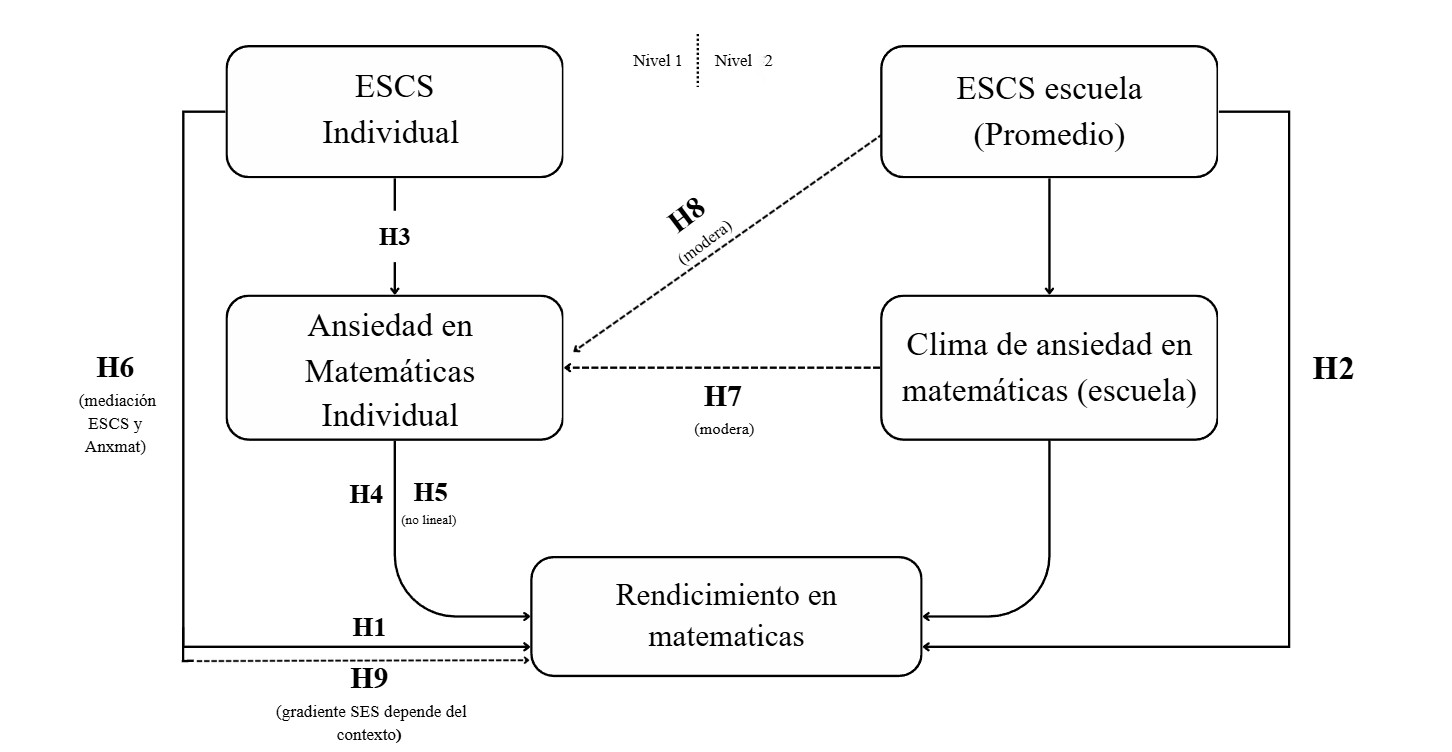
\includegraphics[width=1.1\linewidth,height=\textheight,keepaspectratio]{assets/Imagenes/conceptual_model.jpg}

}

\end{figure}%

\bookmarksetup{startatroot}

\chapter{Metodología}\label{metodologuxeda}

\section{Datos}\label{datos}

La base de datos utilizada en este estudio corresponde al Programa para
la Evaluación Internacional de Estudiantes (PISA) del año 2022. Esta
base es coordinada por la Organización para la Cooperación y el
Desarrollo Económicos (OCDE) y administrada en Chile por el Ministerio
de Educación. PISA evalúa a estudiantes de aproximadamente 15 años
mediante pruebas estandarizadas por computador y cuestionarios de
contexto que recopilan información socioeconómica, emocional y escolar.
Para la presente investigación se trabaja exclusivamente con la
submuestra chilena de PISA 2022, la cual está diseñada mediante un
muestreo probabilístico, estratificado y bietápico. En una primera etapa
se seleccionan escuelas con probabilidad proporcional a su tamaño dentro
de estratos definidos por región, ruralidad y dependencia
administrativa. En una segunda etapa se selecciona aleatoriamente a
estudiantes elegibles dentro de cada escuela, garantizando
representatividad nacional de la población de jóvenes escolarizados de
15 años. Luego de filtrar casos de la submuestra de Chile, La muestra
final utilizada en los análisis es de 6.488 estudiantes, anidados en 230
escuelas a lo largo del país. Esta estructura jerárquica de los datos
sustenta la elección de un modelo multinivel de dos niveles (estudiantes
y escuelas). Como base complementaria, se utilizará el archivo técnico
de PISA 2022 para asegurar la correcta lectura de ponderadores,
variables derivadas y reglas de combinación de los plausible values,
disponibles a través de la OCDE.

\section{Variables}\label{variables}

\subsection{Variable dependiente}\label{variable-dependiente}

La variable dependiente de esta investigación es el rendimiento en
Matemática de los estudiantes de 15 años en Chile. Esta se mide a partir
de los valores plausibles de desempeño en Matemática reportados por PISA
2022, construidos mediante modelos de respuesta al ítem (IRT) y
diseñados para representar la competencia matemática latente de cada
estudiante en la escala internacional de la prueba. Para los análisis
descriptivos se resume la distribución del rendimiento a partir de los
valores plausibles, mientras que en los modelos de regresión multinivel
se siguen las recomendaciones metodológicas de la OCDE para su uso, es
decir, se estiman los modelos separadamente para cada valor plausible y
luego se combinan los resultados obtenidos. De igual manera, en ambos
casos, valores más altos de la escala indican un mejor desempeño en
Matemática.

\subsection{Variables independientes}\label{variables-independientes}

Las variables independientes centrales se organizan en torno a dos
dimensiones: el origen socioeconómico de los estudiantes y la ansiedad
ante Matemáticas, incorporando además sus agregados o promedios a nivel
de escuela como indicadores de composición y clima escolar.

En primer lugar, el nivel socioeconómico individual se mide mediante el
índice socioeconómico, social y cultural de PISA (ESCS), construido a
partir de información sobre el nivel educacional y ocupacional de los
padres, junto con recursos materiales y culturales disponibles en el
hogar. Se trata de un índice continuo estandarizado a nivel
internacional (media cercana a 0 y desviación estándar igual a 1), donde
valores más altos reflejan un origen socioeconómico más ventajoso. En la
muestra chilena, el índice presenta una media aproximada de -0,2 y un
amplio rango de variación entre -4,2 y 2,2, lo que da cuenta de una
fuerte heterogeneidad en las condiciones socioeconómicas del
estudiantado. Este índice se utiliza como principal medida del origen
social de los y las estudiantes.

En segundo lugar, se considera la ansiedad ante Matemáticas como un
mecanismo psicológico clave en la relación entre origen social y
rendimiento académico. Esta se operacionaliza mediante el índice
Mathematics Anxiety (Anxmat), estimado con modelos de respuesta al ítem
utilizando el método Weighted Likelihood Estimate (WLE), que entrega
puntajes continuos estandarizados a partir de las respuestas a múltiples
ítems. que resume la frecuencia e intensidad de emociones negativas
asociadas a situaciones que involucran Matemática. Considerando esto, el
índice es de carácter continuo, con valores centrados en torno a 0, en
la muestra chilena su media se sitúa en torno a 0,5 puntos y su rango va
aproximadamente de -2,4 a 2,6. Valores más altos indican mayores niveles
de ansiedad matemática. Esta variable se entiende como un mecanismo
potencial que puede mediar o modular el efecto del origen socioeconómico
sobre el rendimiento en Matemática.

A nivel de escuela, se incluye el promedio del índice socioeconómico de
los y las estudiantes de cada establecimiento como indicador de la
composición socioeconómica del centro educativo. Este se calcula como el
promedio del índice de todos los estudiantes de la escuela presentes en
la muestra PISA Chile. Valores más altos indican escuelas con una mayor
concentración de estudiantes de origen socioeconómico alto, mientras que
valores más bajos corresponden a establecimientos más desfavorecidos. En
la muestra, el Índice socioeconómico promedio de las escuelas oscila
aproximadamente entre -2,6 y 1,2, con una media cercana a -0,5, lo que
refleja una marcada estratificación entre escuelas. Esta variable
permite capturar efectos de composición y posibles procesos de
segregación escolar, es decir, si más allá del nivel socioeconómico
individual, asistir a escuelas con distinto perfil socioeconómico
promedio se asocia a diferencias en ansiedad y rendimiento en
Matemática.

Finalmente, se incorpora el promedio de ansiedad matemática de la
escuela como indicador del clima emocional frente a la Matemática en
cada establecimiento. Este se obtiene calculando el valor medio del
índice de ansiedad para los estudiantes de cada escuela presentes, y se
interpreta como una medida del clima de ansiedad matemática en el
entorno escolar. En la muestra chilena, esta variable presenta una media
cercana a 0,5 y una desviación estándar de alrededor de 0,4, con valores
que van aproximadamente de -1,7 a 2,2. Valores más altos indican
escuelas donde, en promedio, el estudiantado reporta mayores niveles de
ansiedad frente a la Matemática, mientras que valores más bajos reflejan
un clima emocional menos ansioso. Este indicador permite evaluar si, más
allá de la ansiedad individual, la pertenencia a escuelas con climas de
mayor o menor ansiedad matemática se asocia diferencialmente al
rendimiento en Matemática, capturando así efectos contextuales ligados
al ambiente emocional y a las expectativas en torno a esta asignatura.

\subsection{Variables de control de nivel
individual}\label{variables-de-control-de-nivel-individual}

Además de las variables centrales, se incorporan diversos controles de
nivel individual con el fin de aislar de mejor manera la asociación
entre origen social, ansiedad y rendimiento, evitando atribuir al nivel
socioeconómico o a la ansiedad diferencias que responden a
características sociodemográficas o escolares previas.

En primer lugar, se incluye el género del estudiante, operacionalizado
como una variable dicotómica mujer (1) y hombre (0). En la muestra
chilena la distribución es relativamente equilibrada (51,5\% hombres y
48,5\% mujeres). Esta variable permite controlar por diferencias de
género en ansiedad matemática y rendimiento, ampliamente documentadas en
la literatura.

En segundo lugar, se incorpora un indicador de problemas con el
aprendizaje autodirigido (selfreg), basado en el índice Probself
(Problems with self-directed learning). Este índice continuo recoge
dificultades para organizar el estudio, mantener la concentración,
completar tareas y gestionar de manera autónoma el proceso de
aprendizaje. Valores más altos indican mayores problemas de
autorregulación. Se utiliza como control para no confundir la ansiedad
específica ante Matemática con dificultades generales en el estudio o en
la gestión del tiempo escolar.

En tercer lugar, se considera la repitencia escolar, medida como una
variable dicotómica que distingue entre quienes han repetido al menos un
curso (1) y quienes nunca han repetido (0). En la muestra analizada,
alrededor de un 13\% del estudiantado ha repetido algún curso. Dado que
la repitencia suele estar asociada a trayectorias escolares marcadas por
dificultades de aprendizaje y a contextos socioeconómicos menos
favorecidos, se incluye principalmente como control, reconociendo que se
trata de un resultado previo situado entre la causa y la consecuencia
del bajo rendimiento y la ansiedad.

Adicionalmente, se incorporan dos controles vinculados a la posición
lingüística y migratoria. El primero es si el idioma del hogar es
distinto al idioma de la prueba, codificado como 0 a quienes reportan
hablar español en el hogar (idioma de la prueba en Chile) y como 1 a
quienes declaran otro idioma. En la muestra, aproximadamente un 1,5\% de
los estudiantes se ubica en esta última categoría. Por su parte, el
estatus migrante se codifica como estudiantes de primera o segunda
generación migrante (1) y nativos (0). Cerca de un 6\% del estudiantado
se clasifica como migrante. Ambas variables permiten controlar por
fuentes adicionales de desventaja o diferenciación asociadas a la
condición migratoria y lingüística.

La tabla de descriptivos de nivel individual resume la distribución de
todas estas variables, permitiendo caracterizar la muestra en términos
socioeconómicos, de ansiedad, trayectoria escolar, género,
autorregulación, idioma del hogar y condición migrante.

Para más información, ver el \hyperref[sec-anexo-a]{Apéndice A}.

\begingroup
\footnotesize

\textbf{Figura 3.1. Tabla de descriptivos de nivel individual.}

\begin{longtable}[]{@{}
  >{\raggedright\arraybackslash}p{(\linewidth - 4\tabcolsep) * \real{0.0984}}
  >{\raggedright\arraybackslash}p{(\linewidth - 4\tabcolsep) * \real{0.2323}}
  >{\raggedright\arraybackslash}p{(\linewidth - 4\tabcolsep) * \real{0.6693}}@{}}
\toprule\noalign{}
\begin{minipage}[b]{\linewidth}\raggedright
Variable
\end{minipage} & \begin{minipage}[b]{\linewidth}\raggedright
Etiqueta
\end{minipage} & \begin{minipage}[b]{\linewidth}\raggedright
Resumen estadístico
\end{minipage} \\
\midrule\noalign{}
\endhead
\bottomrule\noalign{}
\endlastfoot
escs (num.) & Índice socioeconómico, social y cultural (ESCS) & Media =
-0.2 (DE = 1.0); mediana = -0.2; min/max = {[}-4.2, 2.2{]}; RI = 1.6 (CV
= -4.1); 5.685 valores distintos; 6.181 casos válidos (95,3 \%) y 307
perdidos (4,7 \%). \\
anxmat (num.) & Ansiedad ante Matemáticas (ANXMAT, WLE) & Media = 0.5
(DE = 1.2); mediana = 0.6; min/max = {[}-2.4, 2.6{]}; RI = 1.3 (CV =
2.1); 167 valores distintos; 5.372 válidos (82,8 \%) y 1.116 perdidos
(17,2 \%). \\
gender\_female (binaria) & Sexo: mujer (=1), hombre (=0) & Proporciones:
0 = 3.343 (51,5 \%); 1 = 3.145 (48,5 \%); media = 0.5; 6.488 válidos
(100 \%) y 0 perdidos (0 \%). \\
selfreg (num.) & Problemas con el aprendizaje autodirigido (PROBSELF,
WLE) & Media = 0.3 (DE = 0.9); mediana = 0.4; min/max = {[}-2.2, 3.1{]};
RI = 1.0 (CV = 3.1); 2.125 valores distintos; 3.106 válidos (47,9 \%) y
3.382 perdidos (52,1 \%). \\
repitencia\_alguna\_vez & Ha repetido al menos un curso (=1) &
Proporciones: 0 = 5.361 (86,8 \%); 1 = 813 (13,2 \%); media = 0.1; 6.174
válidos (95,2 \%) y 314 perdidos (4,8 \%). \\
homelang\_other (binaria) & Idioma del hogar distinto al idioma de la
prueba (=1) & Proporciones: 0 = 6.104 (98,5 \%); 1 = 95 (1,5 \%); media
≈ 0; 6.199 válidos (95,5 \%) y 289 perdidos (4,5 \%). \\
migrante (binaria) & Estudiante migrante (1ª o 2ª generación =1; nativo
= 0) & Proporciones: 0 = 288 (4,8 \%); 1 = 5.756 (95,2 \%); media ≈ 1.0;
6.044 válidos (93,2 \%) y 444 perdidos (6,8 \%). \\
\end{longtable}

\endgroup

\subsection{Variables de control de nivel
escuela}\label{variables-de-control-de-nivel-escuela}

A nivel contextual, además de los promedios de nivel socioeconómico y
ansiedad que constituyen variables de interés, se incorporan ciertas
variables de control que permiten ajustar por características
estructurales e institucionales de los establecimientos.

En primer lugar, se considera el tamaño total de la escuela, que
representa el número total de estudiantes matriculados en el
establecimiento. En la muestra, las escuelas exhiben una gran
variabilidad, con un promedio cercano a 867 estudiantes y valores que
van desde establecimientos pequeños hasta colegios con más de 4.000
estudiantes. Esta variable permite controlar por diferencias
estructurales asociadas al tamaño, potencialmente vinculadas a la
disponibilidad de recursos, al clima escolar y a la organización
pedagógica.

En segundo lugar, se incluye el tipo de establecimiento, construido a
partir de las variables de PISA sobre administración y propiedad,
codificadas en dos categorías principales: escuelas públicas y escuelas
privadas. Aproximadamente tres cuartas partes de los establecimientos de
la muestra corresponden a escuelas públicas y cerca de un cuarto a
escuelas privadas. Esta variable permite considerar diferencias
institucionales y de financiamiento asociadas tanto a la composición
socioeconómica del alumnado como a las oportunidades de aprendizaje en
Matemática.

En tercer lugar, se incorpora un indicador del tipo de comunidad donde
se ubica la escuela, basado en la pregunta que distingue entre distintos
tamaños y tipos de localidades (aldea o zona rural, pueblo pequeño,
ciudad mediana, ciudad grande, megaciudad). Este indicador permite
controlar por el entorno territorial inmediato del establecimiento, que
puede influir en el acceso a recursos educativos, la segregación
residencial y las oportunidades culturales. Para los análisis
descriptivos se presentan las categorías originales de PISA, mientras
que para los modelos estas se agrupan en categorías más parsimoniosas
como rural, urbano pequeño, mediano y urbano grande..

Finalmente, se reporta el número de estudiantes por escuela en la
muestra PISA, que corresponde al tamaño muestral por establecimiento y
no al total de matrícula. Esta variable se utiliza principalmente con
fines descriptivos y para ver variabilidad en el número de estudiantes
por escuela respecto a la evaluación PISA considerando la estructura
multinivel.

A continuacion se presenta la tabla de descriptiva de nivel conextual
que resume la distribucion de todas estas variables.

Para más información, ver el \hyperref[sec-anexo-b]{Apéndice B}.

\textbf{Figura 3.2. Tabla de descriptivos de nivel contextual
(escuelas).} \begingroup \footnotesize   

\begin{longtable}[]{@{}
  >{\raggedright\arraybackslash}p{(\linewidth - 6\tabcolsep) * \real{0.0890}}
  >{\raggedright\arraybackslash}p{(\linewidth - 6\tabcolsep) * \real{0.1957}}
  >{\raggedright\arraybackslash}p{(\linewidth - 6\tabcolsep) * \real{0.6014}}
  >{\raggedright\arraybackslash}p{(\linewidth - 6\tabcolsep) * \real{0.1139}}@{}}
\toprule\noalign{}
\begin{minipage}[b]{\linewidth}\raggedright
Variable
\end{minipage} & \begin{minipage}[b]{\linewidth}\raggedright
Etiqueta
\end{minipage} & \begin{minipage}[b]{\linewidth}\raggedright
Estadísticas / Valores
\end{minipage} & \begin{minipage}[b]{\linewidth}\raggedright
Válido / Perdidos
\end{minipage} \\
\midrule\noalign{}
\endhead
\bottomrule\noalign{}
\endlastfoot
escs\_promedio (num.) & ESCS promedio de la escuela & Media = -0.4 (DE =
0.8); mediana = -0.5; min/max = {[}-2.6, 1.2{]}; RI = 1.2 (CV = -2.1);
230 valores distintos. & 230 (100.0\%) / 0 (0.0\%) \\
anxmat\_promedio (num.) & Ansiedad matemática promedio (ANXMAT, WLE) &
Media = 0.5 (DE = 0.4); mediana = 0.6; min/max = {[}-1.7, 2.2{]}; RI =
0.4 (CV = 0.8); 224 valores distintos. & 224 (97.4\%) / 6 (2.6\%) \\
n\_estudiantes (int) & N.º de estudiantes en la muestra PISA por escuela
& Media = 28.2 (DE = 12.2); mediana = 33; min/max = {[}1, 42{]}; RI =
13.8 (CV = 0.4); 39 valores distintos. & 230 (100.0\%) / 0 (0.0\%) \\
tamano\_escuela (num.) & Tamaño total de la escuela (SCHSIZE) & Media =
866.9 (DE = 611.2); mediana = 743; min/max = {[}25, 4050{]}; RI = 643.5
(CV = 0.7); 205 valores distintos. & 223 (97.0\%) / 7 (3.0\%) \\
tipo\_escuela (factor) & Tipo de establecimiento (público/privado) &
Categorías:private (n = 53; 23.0\%);public (n = 177; 77.0\%). & 230
(100.0\%) / 0 (0.0\%) \\
comunidad\_escolar (factor) & Tipo de comunidad donde se ubica la
escuela (rural/urbano/otro) & Categorías:(1) A village, hamlet or rural
area (n = 6; 2.7\%);(2) A small town (n = 11; 4.9\%);(3) A town (n = 47;
21.0\%);(4) A city (n = 85; 37.9\%);(5) A large city (n = 75;
33.5\%);otras categorías (6--10) ≈ 0\%. & 224 (97.4\%) / 6 (2.6\%) \\
\end{longtable}

Nota. Descriptivos de variables de nivel escuela (N = n.º de escuelas).

\endgroup

Como un ultimo punto respecto a las variables, en los modelos multinivel
todas las variables continuas se trabajan centradas para separar con
claridad los efectos individuales y contextuales. En particular, los
predictores de nivel individual (estudiante) se descomponen en una
componente individual (desviación del valor del estudiante respecto del
promedio de su escuela) y una componente contextual (promedio de la
variable en cada establecimiento). De este modo, la parte individual se
centra en la media del centro educativo, lo que permite interpretar sus
pendientes como efectos estrictamente dentro de escuela, mientras que
sus promedios escolares capturan diferencias entre escuelas
(\citeproc{ref-EndersTofighi2007}{Enders \& Tofighi, 2007};
\citeproc{ref-RaudenbushBryk2002}{Raudenbush \& Bryk, 2002};
\citeproc{ref-SnijdersBosker2012}{Snijders \& Bosker, 2012}).
Adicionalmente, los predictores continuos de nivel contextual se centran
en su media muestral o gran media, facilitando la interpretación de los
interceptos y reduciendo la colinealidad entre términos principales e
interacciones (\citeproc{ref-Bell2019}{Bell et~al., 2019};
\citeproc{ref-EndersTofighi2007}{Enders \& Tofighi, 2007}).

\section{Estrategia de análisis}\label{estrategia-de-anuxe1lisis}

La metodología empleada en esta investigación es de carácter
cuantitativo. El análisis estadístico se realizará en el software R
(versión 4.5.0) (\citeproc{ref-RCoreTeam2024}{R Core Team, 2024}),
utilizando principalmente los paquetes lme4 para la estimación de
modelos multinivel (\citeproc{ref-Bates2015}{Bates et~al., 2015}) y
summarytools para la generación de tablas descriptivas
(\citeproc{ref-Comtois2024}{Comtois, 2024}). Dado que los datos
provienen del estudio PISA 2022, se trabaja con una muestra de
estudiantes de 15 años matriculados en establecimientos escolares en
Chile, lo que implica una estructura jerárquica de estudiantes anidados
en escuelas. Este tipo de estructura hace que las observaciones no sean
independientes entre sí, ya que estudiantes de una misma escuela
comparten recursos, normas, docentes y climas escolares similares. En
estas circunstancias, los modelos de regresión multinivel resultan
especialmente adecuados para analizar cómo un resultado a nivel
individual, en este caso el rendimiento en Matemática, se relaciona con
variables medidas tanto a nivel del estudiante como a nivel de la
escuela (\citeproc{ref-Fairbrother2014}{Fairbrother, 2014};
\citeproc{ref-Hox2017}{Hox et~al., 2017b}).

En términos formales, se estiman modelos de regresión lineal multinivel
de dos niveles con interceptos aleatorios, donde el nivel 1 corresponde
a los y las estudiantes y el nivel 2 a las escuelas. Estos modelos
permiten separar la varianza del rendimiento en Matemática en una
componente individual y una componente entre escuelas, estimar efectos
fijos de las variables independientes en ambos niveles y modelar la
variación aleatoria del intercepto entre establecimientos
(\citeproc{ref-Bell2019}{Bell et~al., 2019}). Como paso inicial, se
estima un modelo nulo (sin predictores) para calcular la correlación
intraclase (ICC), que indica qué proporción de la varianza total del
rendimiento se explica por diferencias entre escuelas. Este diagnóstico
es clave para justificar empíricamente el uso de modelos multinivel y
para dimensionar la importancia de los efectos contextuales
(\citeproc{ref-Aguinis2013}{Aguinis et~al., 2013}).

A partir de este modelo base, se especifica una secuencia de modelos
multinivel orientados a responder las preguntas de investigación y
contrastar las hipótesis planteadas. En primer lugar, se estiman modelos
con efectos directos de nivel individual, incorporando el índice
socioeconómico, social y cultural y el índice de ansiedad ante
Matemáticas como predictores centrales del rendimiento en Matemática,
junto con un conjunto de variables de control individuales: sexo,
problemas con el aprendizaje autodirigido, repitencia de curso, idioma
del hogar distinto al idioma de la prueba y condición migrante. Estos
modelos permiten evaluar en qué medida el rendimiento promedio en
Matemática se asocia con el origen social y la ansiedad matemática de
cada estudiante, controlando por diferencias sociodemográficas y
educativas a nivel individual.

En segundo lugar, se incorporan predictores de nivel escolar con el fin
de capturar efectos contextuales. En particular, se incluyen el nivel
socioeconómico promedio de la escuela como indicador de composición
socioeconómica del establecimiento y el promedio de ansiedad matemática
como indicador del clima de ansiedad ante Matemáticas en la escuela. A
estas variables se suman controles de nivel 2: tamaño del
establecimiento, número de estudiantes de la muestra PISA por escuela,
tipo de establecimiento (público/privado) y tipo de comunidad donde se
ubica la escuela. De este modo, es posible evaluar si el rendimiento en
Matemática se relaciona no sólo con las características individuales del
estudiantado, sino también con las condiciones socioeconómicas y
emocionales promedio de los establecimientos en que estudian
(\citeproc{ref-BayramOzdemir2020}{Bayram-Ozdemir \& Özdemir, 2020};
\citeproc{ref-TrevinoValenzuelaVillalobos2018}{Treviño et~al., 2018}).

Dada la relevancia teórica de los mecanismos de desigualdad y
estratificación escolar, se estiman modelos con interacciones entre
niveles para analizar posibles efectos de moderación
(\citeproc{ref-Hayes2022}{Hayes, 2022}; \citeproc{ref-Hox2017}{Hox
et~al., 2017b}). En particular, se explora si la asociación entre el
origen social individual y el rendimiento varía en función de la
composición socioeconómica de la escuela, así como si la relación entre
la ansiedad matemática individual y el rendimiento depende del clima de
ansiedad promedio del establecimiento. Estas interacciones permiten
evaluar si ciertos entornos escolares amplifican o amortiguan los
efectos de las desventajas socioeconómicas y de la ansiedad matemática
sobre el desempeño en Matemática, articulando así los efectos
individuales y contextuales en una perspectiva plenamente multinivel
(\citeproc{ref-Aguinis2013}{Aguinis et~al., 2013};
\citeproc{ref-Fairbrother2014}{Fairbrother, 2014}).

Finalmente, y con el propósito de explorar la heterogeneidad en el
efecto de la ansiedad matemática entre escuelas, se estiman modelos
multinivel con pendientes aleatorias para la ansiedad matemática a nivel
individual, permitiendo que la asociación entre ansiedad matemática y
rendimiento en Matemática varíe entre establecimientos
(\citeproc{ref-RaudenbushBryk2002}{Raudenbush \& Bryk, 2002};
\citeproc{ref-SnijdersBosker2012}{Snijders \& Bosker, 2012}). La
comparación entre modelos con y sin pendientes aleatorias, mediante
pruebas de razón de verosimilitudes y test de desvianza, permite evaluar
si la inclusión de estas pendientes mejora significativamente el ajuste
del modelo (\citeproc{ref-Bell2019}{Bell et~al., 2019}).

Sobre esta base, se incorporan interacciones de segundo orden entre la
ansiedad matemática individual y características del contexto escolar
(nivel socioeconómico promedio del establecimiento, clima promedio de
ansiedad y tipo de escuela). Esto permite analizar si el efecto negativo
de la ansiedad sobre el rendimiento es más intenso en ciertos tipos de
escuelas, por ejemplo, en establecimientos con alta concentración de
estudiantes de nivel socioeconómico bajo o con climas emocionales más
ansiosos, modelando así la manera en que los contextos escolares pueden
amplificar o atenuar el impacto de la ansiedad matemática sobre el
desempeño (\citeproc{ref-Aguinis2013}{Aguinis et~al., 2013};
\citeproc{ref-EndersTofighi2007}{Enders \& Tofighi, 2007};
\citeproc{ref-Hayes2022}{Hayes, 2022}).

A continuación, se presenta el modelo multinivel propuesto que integra
los efectos individuales y contextuales del nivel socioeconómico y la
ansiedad ante Matemática sobre el rendimiento con pendientes aleatorias
e interacciones cruzadas

\textbf{Figura 3.3:} Modelo multinivel

\[
\begin{aligned}
Y_{ij} &= \gamma_{00}
+ \gamma_{10} ESCS_{ij}
+ \gamma_{20} ANXMAT_{ij}
+ \gamma_{01} \overline{ESCS}_{j}
+ \gamma_{02} \overline{ANXMAT}_{j}
+ \gamma_{03} TYPE_{j} \\
&\quad
+ \gamma_{11}\, ESCS_{ij}\,\overline{ESCS}_{j}
+ \gamma_{21}\, ANXMAT_{ij}\,\overline{ANXMAT}_{j}
+ \gamma_{23}\, ANXMAT_{ij}\,TYPE_{j} \\
&\quad
+ \mathbf{W}_{ij}^{\top}\beta
+ \mathbf{V}_{j}^{\top}\delta \\
&\quad
+ u_{0j}
+ u_{1j} ESCS_{ij}
+ u_{2j} ANXMAT_{ij}
+ e_{ij}.
\end{aligned}
\]

\bookmarksetup{startatroot}

\chapter{Referencias}\label{referencias}

\phantomsection\label{refs}
\begin{CSLReferences}{1}{0}
\bibitem[\citeproctext]{ref-AgenciaCalidad2023Factores2022}
Agencia de Calidad de la Educación. (2023a). \emph{Informe de Resultados
Educativos 2022. Tomo 2: Factores asociados a los resultados
educativos}. Gobierno de Chile, Agencia de Calidad de la Educación.
\url{https://www.agenciaeducacion.cl/}

\bibitem[\citeproctext]{ref-Agencia2023}
Agencia de Calidad de la Educación. (2023b). \emph{Informe Nacional de
Resultados: Sistema de Evaluaci{ó}n de Aprendizajes 2023}. Agencia de
Calidad de la Educaci{ó}n.

\bibitem[\citeproctext]{ref-agencia2023resultados}
Agencia de Calidad de la Educación. (2023c). \emph{Resultados Nacionales
y Factores Asociados: Informe 2023}. Gobierno de Chile.

\bibitem[\citeproctext]{ref-Aguinis2013}
Aguinis, H., Gottfredson, N. M., \& Culpepper, S. A. (2013).
Best-Practice Recommendations for Estimating Cross-Level Interaction
Effects Using Multilevel Modeling. \emph{Journal of Management},
\emph{39}(6), 1490-1528. \url{https://doi.org/10.1177/0149206313478188}

\bibitem[\citeproctext]{ref-de2020peer}
Arruda Raposo, I. P. de, \& Gonçalves, M. B. C. (2020). Peer effects and
educational achievement: Evidence of causal effects using age at school
entry as exogenous variation for Peer quality. \emph{EconomiA},
\emph{21}(1), 18-37.

\bibitem[\citeproctext]{ref-ashcraft2002}
Ashcraft, M. H. (2002). Math anxiety: Personal, educational, and
cognitive consequences. \emph{Current Directions in Psychological
Science}, \emph{11}(5), 181-185.
\url{https://doi.org/10.1111/1467-8721.00196}

\bibitem[\citeproctext]{ref-AshcraftKrause2007}
Ashcraft, M. H., \& Krause, J. A. (2007). Working Memory, Math
Performance, and Math Anxiety. \emph{Psychonomic Bulletin \& Review},
\emph{14}(2), 243-248.

\bibitem[\citeproctext]{ref-ashcraft2009}
Ashcraft, M. H., \& Moore, A. M. (2009). Mathematics anxiety and the
affective drop in performance. \emph{Journal of Psychoeducational
Assessment}, \emph{27}(3), 197-205.
\url{https://doi.org/10.1177/0734282908330580}

\bibitem[\citeproctext]{ref-AshcraftRidley2005}
Ashcraft, M. H., \& Ridley, K. (2005). Math Anxiety and Its Cognitive
Consequences: A Tutorial Review. En J. I. D. Campbell (Ed.), \emph{The
Handbook of Mathematical Cognition} (pp. 315-327). Psychology Press.

\bibitem[\citeproctext]{ref-Atalah2014}
Atalah, E., Cordero, M., Guerra, M. E., Quezada, S., Carrasco, X., \&
Romo, M. (2014). Monitoreo de los indicadores del Programa {«Chile Crece
Contigo»} 2008--2011. \emph{Revista Chilena de Pediatría}, \emph{85}(5),
565-573.
\url{https://www.scielo.cl/scielo.php?script=sci_arttext&pid=S0370-41062014000500007}

\bibitem[\citeproctext]{ref-WorldBank2021Deuda}
Banco Mundial. (2021). \emph{La billonaria deuda con los estudiantes en
pandemia}.
\url{https://www.bancomundial.org/es/news/feature/2021/12/23/la-billonaria-deuda-con-los-estudiantes-en-pandemia}

\bibitem[\citeproctext]{ref-Bandura1997}
Bandura, A. (1997). \emph{Self-Efficacy: The Exercise of Control}. W. H.
Freeman.

\bibitem[\citeproctext]{ref-Barroso2021}
Barroso, C., Ganley, C. M., McGraw, A. L., Geer, E. A., Hart, S. A., \&
Daucourt, M. C. (2021). A meta-analysis of the relation between math
anxiety and math achievement. \emph{Psychological Bulletin},
\emph{147}(2), 134-168. \url{https://doi.org/10.1037/bul0000307}

\bibitem[\citeproctext]{ref-Bates2015}
Bates, D., Mächler, M., Bolker, B., \& Walker, S. (2015). Fitting Linear
Mixed-Effects Models Using {lme4}. \emph{Journal of Statistical
Software}, \emph{67}(1), 1-48.
\url{https://doi.org/10.18637/jss.v067.i01}

\bibitem[\citeproctext]{ref-BayramOzdemir2020}
Bayram-Ozdemir, S., \& Özdemir, M. (2020). The Role of Perceived
Inter-Ethnic Classroom Climate in Adolescents' Engagement in Ethnic
Victimization: For Whom Does It Work? \emph{Journal of Youth and
Adolescence}, \emph{49}(6), 1328-1340.
\url{https://doi.org/10.1007/s10964-020-01228-8}

\bibitem[\citeproctext]{ref-Bell2019}
Bell, A., Fairbrother, M., \& Jones, K. (2019). Fixed and Random Effects
Models: Making an Informed Choice. \emph{Quality \& Quantity},
\emph{53}, 1051-1074. \url{https://doi.org/10.1007/s11135-018-0802-x}

\bibitem[\citeproctext]{ref-Bellei2013}
Bellei, C. (2013). El gran experimento: Mercado y privatizaci{ó}n de la
educaci{ó}n chilena. \emph{Revista de Sociolog{í}a}.

\bibitem[\citeproctext]{ref-BelleiOrellanaCanales2020}
Bellei, C., Orellana, V., \& Canales, M. (2020). Elección de Escuela en
la Clase Alta Chilena. Comunidad, Identidad y Cierre Social.
\emph{Archivos Analíticos de Políticas Educativas}, \emph{28}(5).
\url{https://doi.org/10.14507/epaa.28.3884}

\bibitem[\citeproctext]{ref-inbook}
Bellei, C., Valenzuela, J., \& De los Rios, D. (2010). Segregación
Escolar en Chile. En \emph{Fin de Ciclo: Cambios en la Gobernanza del
Sistema Educativo} (pp. 209-229).

\bibitem[\citeproctext]{ref-Berkowitz2017}
Berkowitz, R., Moore, H., Astor, R. A., \& Benbenishty, R. (2017). A
research synthesis of the associations between socioeconomic background,
inequality, school climate, and academic achievement. \emph{Review of
Educational Research}, \emph{87}(2), 425-469.
\url{https://doi.org/10.3102/0034654316669821}

\bibitem[\citeproctext]{ref-bieg2015}
Bieg, M., Goetz, T., Wolter, I., \& Hall, N. C. (2015). Gender
stereotype endorsement differentially predicts girls' and boys'
trait-state discrepancy in math anxiety. \emph{Frontiers in Psychology},
\emph{6}, 1404. \url{https://doi.org/10.3389/fpsyg.2015.01404}

\bibitem[\citeproctext]{ref-black1998assessment}
Black, P., \& Wiliam, D. (1998). Assessment and Classroom Learning.
\emph{Assessment in Education: Principles, Policy \& Practice},
\emph{5}(1), 7-74.

\bibitem[\citeproctext]{ref-Blok2016}
Blok, L. (2016). \emph{Inequidad en el acceso a la educación superior:
Análisis del Programa Propedéutico de la USACH} {[}Mathesis, Universidad
de Santiago de Chile{]}.
\url{https://www.paiep.usach.cl/sites/paiep/files/documentos/blok_2016_analisis_del_programa_propedeutico.pdf}

\bibitem[\citeproctext]{ref-boaler2019developing}
Boaler, J. (2019). Developing Mathematical Mindsets: The Need to
Interact with Numbers Flexibly and Conceptually. \emph{American
educator}, \emph{42}(4), 28.

\bibitem[\citeproctext]{ref-BorgenZachrissonSandsor2025}
Borgen, N. T., Zachrisson, H. D., \& Sandsør, A. M. J. (2025). \emph{Do
Schools Equalize or Exacerbate Inequality? Between-School Variability in
the Relationship Between Socioeconomic Background and Academic
Achievement}. SocArXiv preprint.
\url{https://osf.io/preprints/socarxiv/tw9r4}

\bibitem[\citeproctext]{ref-Bourdieu1979}
Bourdieu, P. (1979). \emph{La distinción: Criterios y bases sociales del
gusto}. Les Éditions de Minuit.

\bibitem[\citeproctext]{ref-Bourdieu2000}
Bourdieu, P. (2000). \emph{Capital cultural, escuela y espacio social}.
Siglo XXI Editores.

\bibitem[\citeproctext]{ref-BourdieuPasseron1977}
Bourdieu, P., \& Passeron, J.-C. (1977). \emph{La reproduction:
{É}l{é}ments pour une th{é}orie du syst{è}me d'enseignement}. Les
{É}ditions de Minuit.

\bibitem[\citeproctext]{ref-BucareyUgarteUrzua2014}
Bucarey, A., Ugarte, G., \& Urzúa, S. (2014). \emph{El efecto de la
educación preescolar en Chile} {[}Documento de trabajo{]}. CLAPES-UC.
\url{https://s3.us-east-2.amazonaws.com/assets.clapesuc.cl/media_post_4623_eec8ded109.pdf}

\bibitem[\citeproctext]{ref-Budnevich_Portales2020-wq}
Budnevich Portales, C. (2020). \emph{{«La composici{ó}n social de las
escuelas y su relaci{ó}n con el rendimiento acad{é}mico en lenguaje y
matem{á}tica de los estudiantes secundarios chilenos»}}.
\url{https://repositorio.uchile.cl/handle/2250/184386}; Universidad de
Chile.

\bibitem[\citeproctext]{ref-BussoFrisancho2021}
Busso, M., \& Frisancho, V. (2021). \emph{Good Peers Have Asymmetric
Gendered Effects on Female Educational Outcomes: Experimental Evidence
from Mexico} (IDB-WP-1220). Inter-American Development Bank.
\url{https://doi.org/10.18235/0003247}

\bibitem[\citeproctext]{ref-Calarco2020}
Calarco, J. (2020). Avoiding Us versus Them: How Schools' Dependence on
Privileged {«Helicopter»} Parents Influences Class Gaps in Parental
Engagement. \emph{Sociology of Education}, \emph{93}(1), 31-52.
\url{https://doi.org/10.1177/0038040719882325}

\bibitem[\citeproctext]{ref-carey2016}
Carey, E., Devine, A., Hill, F., \& Szűcs, D. (2016). The Chicken or the
Egg? The Direction of the Relationship Between Mathematics Anxiety and
Mathematics Performance. \emph{Frontiers in Psychology}, \emph{6}, 1987.
\url{https://doi.org/10.3389/fpsyg.2015.01987}

\bibitem[\citeproctext]{ref-Carey2019}
Carey, E., Devine, A., Hill, F., \& Szűcs, D. (2019). The Chicken or the
Egg? The Direction of the Relationship between Mathematics Anxiety and
Mathematics Performance. \emph{Frontiers in Psychology}, \emph{10},
1086.

\bibitem[\citeproctext]{ref-Carvajal2022}
Carvajal Monardes, J. (2022). \emph{Malestar emocional en contextos de
desigualdad educativa: experiencias de estudiantes de ense{ñ}anza media
en educaci{ó}n online} {[}Mathesis, Universidad de Chile{]}.
\url{https://repositorio.uchile.cl/handle/2250/193522}

\bibitem[\citeproctext]{ref-repec:eee:injoed:v:92:y:2022:i:c:s0738059322000785}
Ceron, F. I., Bol, T., \& Werfhorst, H. G. van de. (2022). The dynamics
of achievement inequality: The role of performance and choice in Chile.
\emph{International Journal of Educational Development}, \emph{92}(C),
None. \url{https://doi.org/10.1016/j.ijedudev.2022.102628}

\bibitem[\citeproctext]{ref-CeronBolWerfhorst2022}
Cerón, G., Bol, T., \& Werfhorst, H. G. van de. (2022). Socioeconomic
Inequality in Educational Achievement: A Comparative Perspective.
\emph{Comparative Education Review}.

\bibitem[\citeproctext]{ref-Comtois2024}
Comtois, D. (2024). \emph{summarytools: Tools to Quickly and Neatly
Summarize Data}. \url{https://cran.r-project.org/package=summarytools}

\bibitem[\citeproctext]{ref-Delgado-Floody2024-dw}
Delgado-Floody, P., Cristi-Montero, C., Jerez-Mayorga, D., Ruiz-Ariza,
A., Guzmán-Guzmán, I. P., Álvarez, C., Gómez-López, M.,
Carter-Thuillier, B., \& Caamaño-Navarrete, F. (2024). Exploring the
mediating role of promoting school physical activity on the relationship
between low socioeconomic status and academic achievement and school
climate: evidence from 4,990 Chilean schools. \emph{Front. Public
Health}, \emph{12}, 1426108.

\bibitem[\citeproctext]{ref-devine2012}
Devine, A., Fawcett, K., Szűcs, D., \& Dowker, A. (2012). Gender
differences in mathematics anxiety and the relation to mathematics
performance while controlling for test anxiety. \emph{Behavioral and
Brain Functions}, \emph{8}(1), 33.
\url{https://doi.org/10.1186/1744-9081-8-33}

\bibitem[\citeproctext]{ref-DIPRES2012ChCC}
Dirección de Presupuestos. (2012). \emph{Evaluación de Impacto del
Sistema de Protección Integral a la Infancia {«Chile Crece Contigo»}}.
Ministerio de Hacienda, Gobierno de Chile.
\url{https://www.dipres.gob.cl/597/articles-189318_informe_final.pdf}

\bibitem[\citeproctext]{ref-Dowker2016}
Dowker, A., Sarkar, A., \& Looi, C. I. (2016). Mathematics Anxiety: What
Have We Learned in 60 Years? \emph{Frontiers in Psychology}, \emph{7},
508.

\bibitem[\citeproctext]{ref-EndersTofighi2007}
Enders, C. K., \& Tofighi, D. (2007). Centering Predictor Variables in
Cross-Sectional Multilevel Models: A New Look at an Old Issue.
\emph{Psychological Methods}, \emph{12}(2), 121-138.
\url{https://doi.org/10.1037/1082-989X.12.2.121}

\bibitem[\citeproctext]{ref-Eysenck2007}
Eysenck, M. W., Derakshan, N., Santos, R., \& Calvo, M. G. (2007).
Anxiety and Cognitive Performance: Attentional Control Theory.
\emph{Emotion}, \emph{7}(2), 336-353.

\bibitem[\citeproctext]{ref-Fairbrother2014}
Fairbrother, M. (2014). Two Multilevel Modeling Techniques for Analyzing
Comparative Longitudinal Survey Datasets. \emph{Political Science
Research and Methods}, \emph{2}(1), 119-140.
\url{https://doi.org/10.1017/psrm.2013.24}

\bibitem[\citeproctext]{ref-FalabellaDeLaVega2016}
Falabella, A., \& Vega, L. F. D. la. (2016). Pol{í}ticas de
responsabilizaci{ó}n por desempe{ñ}o escolar: Un debate a partir de la
literatura internacional y el caso chileno. \emph{Estudios
Pedag{ó}gicos}, \emph{42}(2), 395-413.
\url{https://doi.org/10.4067/S0718-07052016000200023}

\bibitem[\citeproctext]{ref-fraser2012classroom}
Fraser, B. J. (2012). Classroom Learning Environments: Retrospect,
Context, and Prospect. En B. J. Fraser, K. Tobin, \& C. J. McRobbie
(Eds.), \emph{Second International Handbook of Science Education} (pp.
1191-1239). Springer.

\bibitem[\citeproctext]{ref-geary2021class}
Geary, D. C., Hoard, M. K., Nugent, L., \& Scofield, J. E. (2021).
In-class attention, spatial ability, and mathematics anxiety predict
across-grade gains in adolescents' mathematics achievement.
\emph{Journal of educational psychology}, \emph{113}(4), 754.

\bibitem[\citeproctext]{ref-Global_Education_Monitoring_Report_Team2020-xq}
Global Education Monitoring Report Team, Laboratory of Education
Research and Innovation for Latin America and the Caribbean, \& UNESCO
Office Santiago and Regional Bureau for Education in Latin America and
the Caribbean. (2020). \emph{Global Education Monitoring Report: Latin
America and the Caribbean - Education and inclusion}. UNESCO Publishing.

\bibitem[\citeproctext]{ref-goetz2013}
Goetz, T., Bieg, M., Lüdtke, O., Pekrun, R., \& Hall, N. C. (2013). Do
girls really experience more anxiety in mathematics? \emph{Psychological
Science}, \emph{24}(10), 2079-2087.
\url{https://doi.org/10.1177/0956797613486989}

\bibitem[\citeproctext]{ref-article1}
González, I., Espinosa, J., \& Soledad, G. (2025). Construcción y
Validación del Instrumento de Medición {«Ansiedad Generalizada en
Matemáticas»} para Estudiantes de Bachillerato de la Universidad de
Guadalajara: Construction and Validation of the Measuring Instrument
{«Generalized Anxiety in Mathematics»} for High School Students at the
University of Guadalajara. \emph{LATAM Revista Latinoamericana de
Ciencias Sociales y Humanidades}, \emph{6}.
\url{https://doi.org/10.56712/latam.v6i2.3771}

\bibitem[\citeproctext]{ref-guo2025sesreview}
Guo, Z. (2025). Family Socioeconomic Status and Academic Achievement: A
Narrative Review of Mechanisms and Contexts. \emph{Educational Review}.

\bibitem[\citeproctext]{ref-Gutiuxe9rrez02012023}
Gutiérrez, G. (2023). Is it socioeconomic or academic? Disentangling
sources of peer effects on student achievement. \emph{British Journal of
Sociology of Education}, \emph{44}(1), 144-163.
\url{https://doi.org/10.1080/01425692.2022.2137465}

\bibitem[\citeproctext]{ref-HascoetGiaconiJamain2021}
Hascoët, M., Giaconi, V., \& Jamain, L. (2021). Family socioeconomic
status and parental expectations affect mathematics achievement in a
national sample of Chilean students. \emph{International Journal of
Behavioral Development}, \emph{45}(2), 122-132.
\url{https://doi.org/10.1177/0165025420965731}

\bibitem[\citeproctext]{ref-hattie2009visible}
Hattie, J. (2009a). \emph{Visible Learning: A Synthesis of over 800
Meta-Analyses Relating to Achievement}. Routledge.

\bibitem[\citeproctext]{ref-Hattie2009}
Hattie, J. (2009b). \emph{Visible Learning: A Synthesis of Over 800
Meta-Analyses Relating to Achievement}. Routledge.

\bibitem[\citeproctext]{ref-Hayes2022}
Hayes, A. F. (2022). \emph{Introduction to Mediation, Moderation, and
Conditional Process Analysis: A Regression-Based Approach} (3.ª ed.).
The Guilford Press.

\bibitem[\citeproctext]{ref-hembree1990}
Hembree, R. (1990a). The nature, effects, and relief of mathematics
anxiety. \emph{Journal for Research in Mathematics Education},
\emph{21}(1), 33-46. \url{https://doi.org/10.2307/749455}

\bibitem[\citeproctext]{ref-Hembree1990}
Hembree, R. (1990b). The Nature, Effects, and Relief of Mathematics
Anxiety. \emph{Journal for Research in Mathematics Education},
\emph{21}(1), 33-46.

\bibitem[\citeproctext]{ref-hopko2003}
Hopko, D. R., Mahadevan, R., Bare, R. L., \& Hunt, M. K. (2003). The
Abbreviated Math Anxiety Scale (AMAS): Construction, validity, and
reliability. \emph{Assessment}, \emph{10}(2), 178-182.
\url{https://doi.org/10.1177/1073191103010002008}

\bibitem[\citeproctext]{ref-hox2017multilevel}
Hox, J. J., Moerbeek, M., \& Schoot, R. van de. (2017a).
\emph{Multilevel Analysis: Techniques and Applications} (3.ª ed.).
Routledge.

\bibitem[\citeproctext]{ref-Hox2017}
Hox, J. J., Moerbeek, M., \& Schoot, R. van de. (2017b).
\emph{Multilevel Analysis: Techniques and Applications} (3.ª ed.).
Routledge.

\bibitem[\citeproctext]{ref-HuangLiu2025}
Huang, M., \& Liu, X. (2025). Pathways to equity: A mediation analysis
of gender, SES, and mathematics achievement using PISA 2022 UK data.
\emph{International Journal of Educational Research}, \emph{133},
102666. \url{https://doi.org/10.1016/j.ijer.2025.102666}

\bibitem[\citeproctext]{ref-hyde1990}
Hyde, J. S., Fennema, E., Ryan, M., Frost, L. A., \& Hopp, C. (1990).
Gender comparisons of mathematics attitudes and affect: A meta-analysis.
\emph{Psychology of Women Quarterly}, \emph{14}(3), 299-324.
\url{https://doi.org/10.1111/j.1471-6402.1990.tb00022.x}

\bibitem[\citeproctext]{ref-Jakubowski2025-qv}
Jakubowski, M., Gajderowicz, T., \& Patrinos, H. A. (2025). {COVID-19},
school closures, and student learning outcomes. New global evidence from
{PISA}. \emph{NPJ Sci. Learn.}, \emph{10}(1), 5.
\url{https://www.nature.com/articles/s41539-025-00297-3\#citeas}

\bibitem[\citeproctext]{ref-Kersha2020}
Kersha, Y. (2020). School Socioeconomic Composition as a Factor of
Educational Inequality Reproduction. \emph{Voprosy Obrazovaniya /
Educational Studies Moscow}, \emph{2020}(4), 85-112.
\url{https://doi.org/10.17323/1814-9545-2020-4-85-112}

\bibitem[\citeproctext]{ref-Lareau2003}
Lareau, A. (2003). \emph{Unequal Childhoods: Class, Race, and Family
Life}. University of California Press.

\bibitem[\citeproctext]{ref-Lau2022}
Lau, N. T. T., Rubinsten, O., Lee, M. W., \& Ansari, D. (2022).
Disentangling the individual and contextual effects of math anxiety: A
multilevel analysis of 15-year-old students across 65 countries.
\emph{Proceedings of the National Academy of Sciences}, \emph{119}(14),
e2115855119. \url{https://doi.org/10.1073/pnas.2115855119}

\bibitem[\citeproctext]{ref-LinDurbinRancer2017}
Lin, Y., Durbin, J. M., \& Rancer, A. S. (2017). Perceived Instructor
Argumentativeness, Verbal Aggressiveness, and Classroom Communication
Climate in Relation to Student State Motivation and Math Anxiety.
\emph{Communication Education}, \emph{66}(3), 330-349.
\url{https://doi.org/10.1080/03634523.2016.1245427}

\bibitem[\citeproctext]{ref-madjar2018predictors}
Madjar, N., Zalsman, G., Weizman, A., Lev-Ran, S., \& Shoval, G. (2018).
Predictors of developing mathematics anxiety among middle-school
students: A 2-year prospective study. \emph{International Journal of
Psychology}, \emph{53}(6), 426-432.

\bibitem[\citeproctext]{ref-MaloneyBeilock2012}
Maloney, E. A., \& Beilock, S. L. (2012). Math Anxiety: Who Has It, Why
It Develops, and How To Guard against It. \emph{Trends in Cognitive
Sciences}, \emph{16}(8), 404-406.

\bibitem[\citeproctext]{ref-MarshHau2003}
Marsh, H. W., \& Hau, K.-T. (2003). Big-Fish-Little-Pond Effect on
Academic Self-Concept: A Cross-Cultural (26-Country) Test of the
Negative Effects of Academically Selective Schools. \emph{American
Psychologist}, \emph{58}(5), 364-376.
\url{https://doi.org/10.1037/0003-066X.58.5.364}

\bibitem[\citeproctext]{ref-Martin-Puga2022-fg}
Martı́n-Puga, M. E., Justicia-Galiano, M. J., Gómez-Pérez, M. M., \&
Pelegrina, S. (2022). Psychometric properties, factor structure, and
gender and educational level invariance of the Abbreviated Math Anxiety
Scale ({AMAS}) in Spanish children and adolescents. \emph{Assessment},
\emph{29}(3), 425-440.

\bibitem[\citeproctext]{ref-MenesesOrtegaKuzmanicValenzuela2025}
Meneses, A., Ortega, L., Kuzmanic, D., \& Valenzuela, J. P. (2025).
Desigualdades socioecon{ó}micas en el SIMCE de Matem{á}tica: efectos
individuales, escolares y de contexto. \emph{Revista a definir}.

\bibitem[\citeproctext]{ref-mineduc2023pisa}
Ministerio de Educación de Chile, \& Unidad de Currículum y Evaluación.
(2023). \emph{PISA 2022: Informe Nacional Chile}. MINEDUC.

\bibitem[\citeproctext]{ref-mizala2012chile}
Mizala, A., \& Torche, F. (2012). Bringing the Schools Back In:
Stratification of Educational Achievement in the Chilean Voucher System.
\emph{International Journal of Educational Development}, \emph{32}(1),
132-144.

\bibitem[\citeproctext]{ref-Neuman2022}
Neuman, M. (2022). PISA data clusters reveal student and school
inequality that affects results. \emph{PLOS ONE}, \emph{17}(5),
e0267040. \url{https://doi.org/10.1371/journal.pone.0267040}

\bibitem[\citeproctext]{ref-OHara2022}
O'Hara, G., Kennedy, H., Naoufal, M., \& Montreuil, T. (2022). The role
of the classroom learning environment in students' mathematics anxiety:
A scoping review. \emph{British Journal of Educational Psychology},
\emph{92}(4), 1458-1486. \url{https://doi.org/10.1111/bjep.12510}

\bibitem[\citeproctext]{ref-oecd2023chile}
OECD. (2023a). \emph{PISA 2022 Country Note: Chile}. OECD Publishing.

\bibitem[\citeproctext]{ref-oecd2023pisa}
OECD. (2023b). \emph{PISA 2022 Results: Student Performance, Equity and
Well-Being}. OECD Publishing.

\bibitem[\citeproctext]{ref-OECD2023b}
OECD. (2023c). \emph{PISA 2022 Results. Volume II: Learning During and
After COVID-19}. OECD Publishing. \url{https://www.oecd.org}

\bibitem[\citeproctext]{ref-OECD2025TeacherSupport}
OECD. (2025). \emph{Teacher Support for Student Learning: Insights from
PISA}. Organisation for Economic Co-operation; Development.
\url{https://www.oecd.org/content/dam/oecd/en/publications/reports/2025/06/teacher-support-for-student-learning_1433548a/97b3a899-en.pdf}

\bibitem[\citeproctext]{ref-Ortega2023-fi}
Ortega, P. J. (2023). Factores Asociados al Rendimiento en Matem{á}ticas
de Estudiantes Espa{ñ}oles en Educaci{ó}n Primaria. \emph{REICE Rev.
Iberoam. Sobre Calid. Efic. Cambio Educ.}, \emph{21}(3), 175-191.

\bibitem[\citeproctext]{ref-OteroCarranzaContreras2021}
Otero, G., Carranza, R., \& Contreras, D. (2021). Spatial Divisions of
Poverty and Wealth: Does Segregation Affect Educational Achievement?
\emph{Socio-Economic Review}, \emph{21}(1), 617-641.
\url{https://doi.org/10.1093/ser/mwab022}

\bibitem[\citeproctext]{ref-pekrun2006}
Pekrun, R. (2006b). The control-value theory of achievement emotions:
Assumptions, corollaries, and implications for educational research and
practice. \emph{Educational Psychology Review}, \emph{18}(4), 315-341.
\url{https://doi.org/10.1007/s10648-006-9029-9}

\bibitem[\citeproctext]{ref-Pekrun2006}
Pekrun, R. (2006a). The Control-Value Theory of Achievement Emotions:
Assumptions, Corollaries, and Implications for Educational Research and
Practice. \emph{Educational Psychology Review}, \emph{18}(4), 315-341.

\bibitem[\citeproctext]{ref-Pintrich2004}
Pintrich, P. R. (2004). A Conceptual Framework for Assessing Motivation
and Self-Regulated Learning in College Students. \emph{Educational
Psychology Review}, \emph{16}(4), 385-407.

\bibitem[\citeproctext]{ref-Qiu2022}
Qiu, F. (2022). Reviewing the role of positive classroom climate in
improving English as a foreign language students' social interactions in
the online classroom. \emph{Frontiers in Psychology}, \emph{13},
1012524. \url{https://doi.org/10.3389/fpsyg.2022.1012524}

\bibitem[\citeproctext]{ref-RCoreTeam2024}
R Core Team. (2024). \emph{R: A Language and Environment for Statistical
Computing}. R Foundation for Statistical Computing.
\url{https://www.R-project.org/}

\bibitem[\citeproctext]{ref-RamirezShawMaloney2018}
Ramirez, G., Shaw, S. T., \& Maloney, E. A. (2018). Math Anxiety: Past
Research, Promising Interventions, and a New Interpretation Framework.
\emph{Educational Psychologist}, \emph{53}(3), 145-164.
\url{https://doi.org/10.1080/00461520.2018.1447384}

\bibitem[\citeproctext]{ref-RaudenbushBryk2002}
Raudenbush, S. W., \& Bryk, A. S. (2002). \emph{Hierarchical Linear
Models: Applications and Data Analysis Methods} (2.ª ed.). Sage.

\bibitem[\citeproctext]{ref-richardson1972}
Richardson, F. C., \& Suinn, R. M. (1972). The mathematics anxiety
rating scale: Psychometric data. \emph{Journal of Counseling
Psychology}, \emph{19}(6), 551-554.
\url{https://doi.org/10.1037/h0033456}

\bibitem[\citeproctext]{ref-10.1093ux2fesrux2fjcae031}
Rosenqvist, E., \& Brandén, M. (2024). School composition and academic
decisions. \emph{European Sociological Review}, \emph{41}(2), 232-247.
\url{https://doi.org/10.1093/esr/jcae031}

\bibitem[\citeproctext]{ref-article}
Rubie-Davies, C. (2009). Teacher expectations and perceptions of student
attributes: Is there a relationship? \emph{The British journal of
educational psychology}, \emph{80}, 121-135.
\url{https://doi.org/10.1348/000709909X466334}

\bibitem[\citeproctext]{ref-Sammallahti2023}
Sammallahti, E., Finell, J., Jonsson, B., \& Korhonen, J. (2023). A
Meta-Analysis of Math Anxiety Interventions. \emph{Journal of Numerical
Cognition}, \emph{9}(2), 346-362. \url{https://doi.org/10.5964/jnc.8401}

\bibitem[\citeproctext]{ref-SnijdersBosker2012}
Snijders, T. A. B., \& Bosker, R. J. (2012). \emph{Multilevel Analysis:
An Introduction to Basic and Advanced Multilevel Modeling} (2.ª ed.).
Sage.

\bibitem[\citeproctext]{ref-Stella2021}
Stella, M. (2021). Network Psychometrics and Cognitive Network Science
Open New Ways for Detecting, Understanding and Tackling the Complexity
of Math Anxiety: A Review. \emph{arXiv}.
\url{https://doi.org/10.48550/arXiv.2108.13800}

\bibitem[\citeproctext]{ref-szucs2020}
Szűcs, D., \& Mammarella, I. C. (2020). \emph{Math Anxiety}.
International Bureau of Education, UNESCO, Educational Practices Series.
\url{https://www.ibe.unesco.org/en}

\bibitem[\citeproctext]{ref-TianHuiLei2025}
Tian, L., Hui, N., \& Lei, H. (2025). Teacher Feedback Quality,
Self-Regulated Learning, and Mathematics Anxiety: A Structural Equation
Modeling Approach. \emph{Learning and Instruction}.

\bibitem[\citeproctext]{ref-TrevinoValenzuelaVillalobos2018}
Treviño, E., Valenzuela, J. P., Villalobos, C., \& Béjares, C. (2018).
Agrupamiento por habilidad acad{é}mica en el sistema escolar: nueva
evidencia para comprender las desigualdades del sistema educativo
chileno. \emph{Revista Mexicana de Investigaci{ó}n Educativa},
\emph{23}(76), 45-71.
\url{https://www.scielo.org.mx/pdf/rmie/v23n76/1405-6666-rmie-23-76-45.pdf}

\bibitem[\citeproctext]{ref-UNESCO2020}
UNESCO. (2020). \emph{Global Education Monitoring Report 2020: Inclusion
and education: All means all}. UNESCO.

\bibitem[\citeproctext]{ref-Valenzuela2014}
Valenzuela, J. P., Bellei, C., \& Ríos, D. de los. (2014). Segregaci{ó}n
escolar en Chile. En C. Bellei, D. Carrasco, \& J. P. Valenzuela (Eds.),
\emph{Ecos de la revoluci{ó}n ping{ü}ina} (pp. 257-292). LOM.

\bibitem[\citeproctext]{ref-VANDEWERFHORST201822}
van de Werfhorst, H. G. (2018). Early tracking and socioeconomic
inequality in academic achievement: Studying reforms in nine countries.
\emph{Research in Social Stratification and Mobility}, \emph{58}, 22-32.
https://doi.org/\url{https://doi.org/10.1016/j.rssm.2018.09.002}

\bibitem[\citeproctext]{ref-WangDegol2016}
Wang, M.-T., \& Degol, J. L. (2016). School Climate: A Review of the
Construct, Measurement, and Impact on Student Outcomes.
\emph{Educational Psychology Review}, \emph{28}(2), 315-352.
\url{https://doi.org/10.1007/s10648-015-9319-1}

\bibitem[\citeproctext]{ref-Willms1986}
Willms, J. D. (1986). Social Class Segregation and Its Relationship to
Pupils' Examination Results in Scotland. \emph{American Sociological
Review}.

\bibitem[\citeproctext]{ref-Willms2010}
Willms, J. D. (2010). School Composition and Contextual Effects on
Student Outcomes. \emph{Teachers College Record}, \emph{112}(4),
1008-1037.

\bibitem[\citeproctext]{ref-Young2012}
Young, C. B., Wu, S. S., \& Menon, V. (2012a). The Neurodevelopmental
Basis of Math Anxiety. \emph{Psychological Science}, \emph{23}(5),
492-501. \url{https://doi.org/10.1177/0956797611429134}

\bibitem[\citeproctext]{ref-young2012}
Young, C. B., Wu, S., \& Menon, V. (2012b). The neurodevelopmental basis
of math anxiety. \emph{Psychological Science}, \emph{23}(5), 492-501.
\url{https://doi.org/10.1177/0956797611429134}

\bibitem[\citeproctext]{ref-YoussefAlibraheim2025}
Youssef, A., \& Alibraheim, M. (2025). Self-Regulated Learning
Strategies and Anxiety in Quantitative Courses. \emph{Journal of
Educational Psychology}.

\bibitem[\citeproctext]{ref-Zimmerman2000}
Zimmerman, B. J. (2000). Attaining Self-Regulation: A Social Cognitive
Perspective. \emph{Handbook of Self-Regulation}, 13-39.

\end{CSLReferences}

\cleardoublepage
\phantomsection
\addcontentsline{toc}{part}{Apéndices}
\appendix

\chapter{Estadísticos descriptivos -- Nivel 1}\label{sec-anexo-a}

\begingroup
\footnotesize

\textbf{Tabla A. Estadísticos descriptivos -- Nivel 1 (estudiantes)}

\begin{longtable}[]{@{}
  >{\raggedright\arraybackslash}p{(\linewidth - 16\tabcolsep) * \real{0.5678}}
  >{\raggedleft\arraybackslash}p{(\linewidth - 16\tabcolsep) * \real{0.0424}}
  >{\raggedleft\arraybackslash}p{(\linewidth - 16\tabcolsep) * \real{0.0508}}
  >{\raggedleft\arraybackslash}p{(\linewidth - 16\tabcolsep) * \real{0.0508}}
  >{\raggedleft\arraybackslash}p{(\linewidth - 16\tabcolsep) * \real{0.0678}}
  >{\raggedleft\arraybackslash}p{(\linewidth - 16\tabcolsep) * \real{0.0593}}
  >{\raggedleft\arraybackslash}p{(\linewidth - 16\tabcolsep) * \real{0.0593}}
  >{\raggedleft\arraybackslash}p{(\linewidth - 16\tabcolsep) * \real{0.0508}}
  >{\raggedleft\arraybackslash}p{(\linewidth - 16\tabcolsep) * \real{0.0508}}@{}}
\toprule\noalign{}
\begin{minipage}[b]{\linewidth}\raggedright
Variable
\end{minipage} & \begin{minipage}[b]{\linewidth}\raggedleft
N
\end{minipage} & \begin{minipage}[b]{\linewidth}\raggedleft
Mín.
\end{minipage} & \begin{minipage}[b]{\linewidth}\raggedleft
P25
\end{minipage} & \begin{minipage}[b]{\linewidth}\raggedleft
Mediana
\end{minipage} & \begin{minipage}[b]{\linewidth}\raggedleft
Media
\end{minipage} & \begin{minipage}[b]{\linewidth}\raggedleft
P75
\end{minipage} & \begin{minipage}[b]{\linewidth}\raggedleft
Máx.
\end{minipage} & \begin{minipage}[b]{\linewidth}\raggedleft
DE
\end{minipage} \\
\midrule\noalign{}
\endhead
\bottomrule\noalign{}
\endlastfoot
Índice socioeconómico, social y cultural (ESCS) & 6181 & -4.22 & -0.99 &
-0.21 & -0.24 & 0.58 & 2.24 & 1.00 \\
Ansiedad ante Matemáticas (ANXMAT, WLE) & 5372 & -2.39 & -0.12 & 0.57 &
0.55 & 1.14 & 2.63 & 1.16 \\
Sexo: mujer (=1), hombre (=0) & 6488 & 0.00 & 0.00 & 0.00 & 0.48 & 1.00
& 1.00 & 0.50 \\
Problemas con el aprendizaje autodirigido (PROBSELF, WLE) & 3106 & -2.23
& -0.13 & 0.41 & 0.30 & 0.89 & 3.10 & 0.95 \\
Ha repetido al menos un curso (=1) & 6174 & 0.00 & 0.00 & 0.00 & 0.13 &
0.00 & 1.00 & 0.34 \\
Idioma del hogar distinto al idioma de la prueba (=1) & 6199 & 0.00 &
0.00 & 0.00 & 0.02 & 0.00 & 1.00 & 0.12 \\
Estudiante migrante (1ª o 2ª generación =1; nativo = 0) & 6044 & 0.00 &
1.00 & 1.00 & 0.95 & 1.00 & 1.00 & 0.21 \\
\end{longtable}

\endgroup

\chapter{Estadísticos descriptivos -- Nivel 2}\label{sec-anexo-b}

\begingroup
\footnotesize

\textbf{Tabla B. Estadísticos descriptivos -- Nivel 2 (escuelas)}

\begin{longtable}[]{@{}
  >{\raggedright\arraybackslash}p{(\linewidth - 16\tabcolsep) * \real{0.5263}}
  >{\raggedleft\arraybackslash}p{(\linewidth - 16\tabcolsep) * \real{0.0439}}
  >{\raggedleft\arraybackslash}p{(\linewidth - 16\tabcolsep) * \real{0.0614}}
  >{\raggedleft\arraybackslash}p{(\linewidth - 16\tabcolsep) * \real{0.0614}}
  >{\raggedleft\arraybackslash}p{(\linewidth - 16\tabcolsep) * \real{0.0702}}
  >{\raggedleft\arraybackslash}p{(\linewidth - 16\tabcolsep) * \real{0.0614}}
  >{\raggedleft\arraybackslash}p{(\linewidth - 16\tabcolsep) * \real{0.0614}}
  >{\raggedleft\arraybackslash}p{(\linewidth - 16\tabcolsep) * \real{0.0526}}
  >{\raggedleft\arraybackslash}p{(\linewidth - 16\tabcolsep) * \real{0.0614}}@{}}
\toprule\noalign{}
\begin{minipage}[b]{\linewidth}\raggedright
Variable
\end{minipage} & \begin{minipage}[b]{\linewidth}\raggedleft
N
\end{minipage} & \begin{minipage}[b]{\linewidth}\raggedleft
Mín.
\end{minipage} & \begin{minipage}[b]{\linewidth}\raggedleft
P25
\end{minipage} & \begin{minipage}[b]{\linewidth}\raggedleft
Mediana
\end{minipage} & \begin{minipage}[b]{\linewidth}\raggedleft
Media
\end{minipage} & \begin{minipage}[b]{\linewidth}\raggedleft
P75
\end{minipage} & \begin{minipage}[b]{\linewidth}\raggedleft
Máx.
\end{minipage} & \begin{minipage}[b]{\linewidth}\raggedleft
DE
\end{minipage} \\
\midrule\noalign{}
\endhead
\bottomrule\noalign{}
\endlastfoot
ESCS promedio de la escuela & 230 & -2.59 & -0.95 & -0.47 & -0.37 & 0.22
& 1.21 & 0.78 \\
Ansiedad matemática promedio de la escuela (ANXMAT, WLE) & 224 & -1.67 &
0.32 & 0.56 & 0.54 & 0.77 & 2.23 & 0.44 \\
N.º de estudiantes en la muestra PISA por escuela & 230 & 1.00 & 23.25 &
33.00 & 28.21 & 37.00 & 42.00 & 12.23 \\
Tamaño total de la escuela (matrícula, SCHSIZE) & 223 & 25.00 & 458.50 &
743.00 & 866.95 & 1102.00 & 4050.00 & 611.16 \\
\end{longtable}

\endgroup


\backmatter

% --- Cuerpo del libro (capítulos) en arábigos ---
\mainmatter
\pagestyle{scrheadings}

% --- (Opcional) Estilo del índice general ---
% \addtocontents{toc}{\protect\thispagestyle{plain}}


\end{document}
